\chapter{Кликни и победи}

В този проект двата героя се придвижват напред, когато играчът клика върху синия или червения бутон. Колкото по- бързо играчът клика върху бутона, толкова по- бързо неговият герой се придвижва напред. Печели този играч, който първи достигне до зелената финална линия.

\begin{figure}[H]
  \centering
  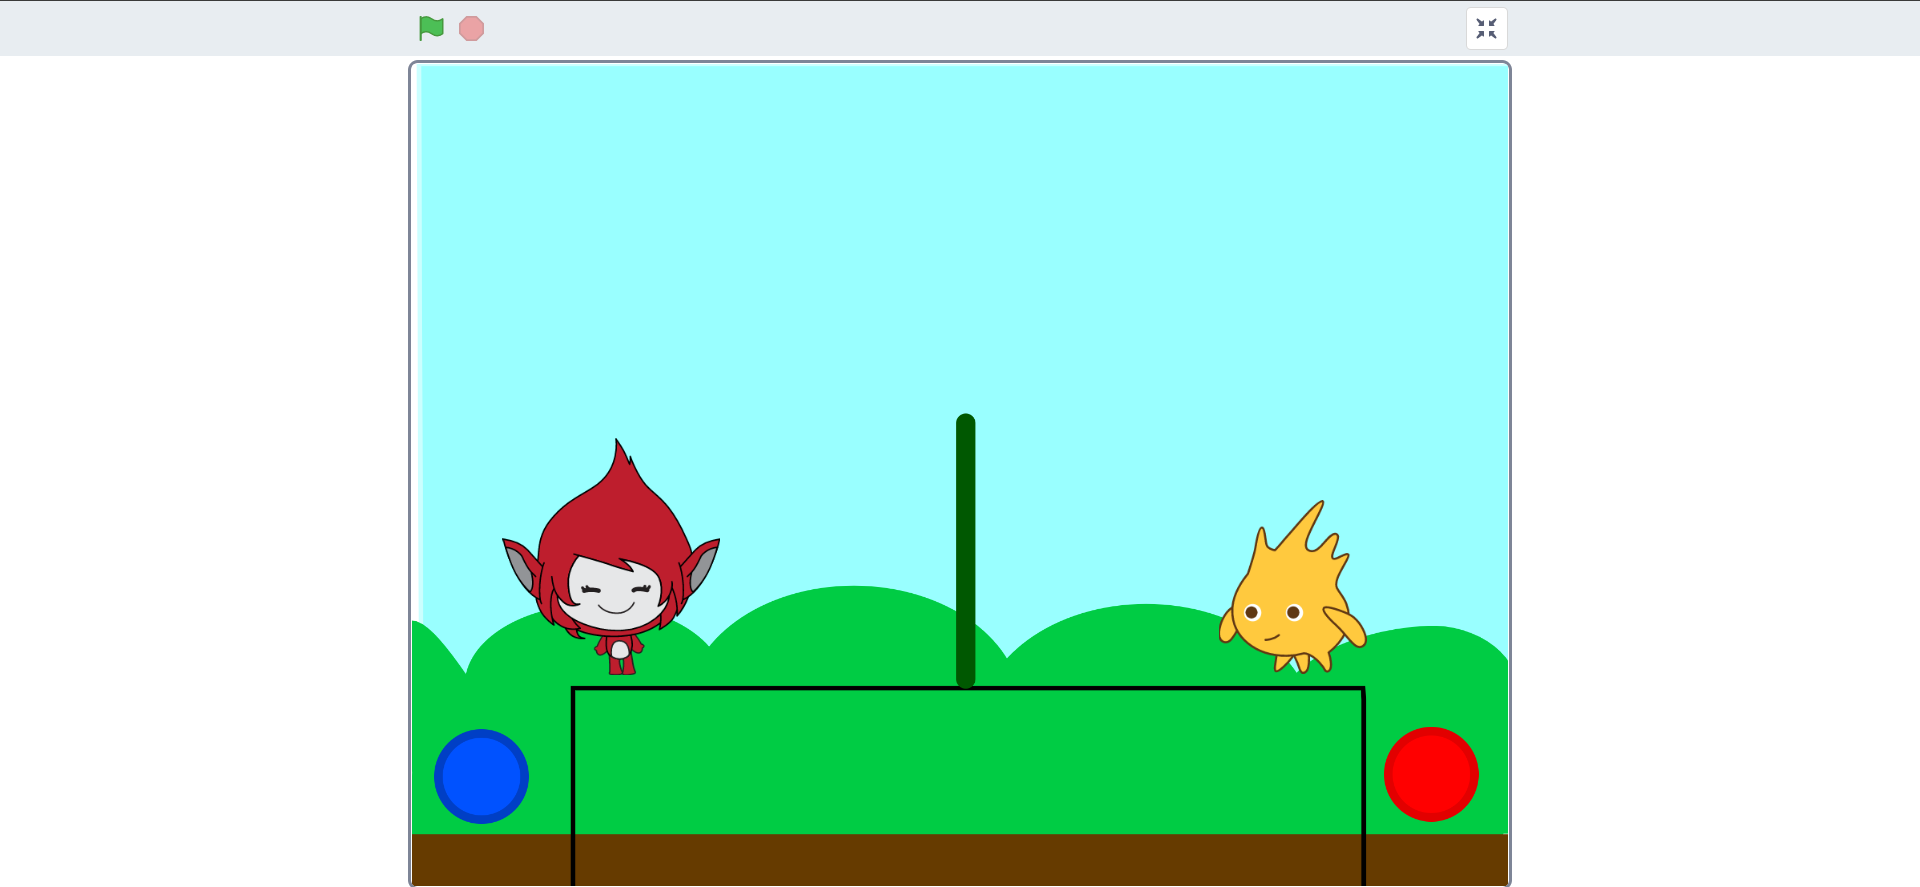
\includegraphics[width=1.0\linewidth,height=0.5\linewidth]{fig030001.png}
  \caption{Кликни и победи}
\label{fig030001}
\end{figure}

\section{Добавяне на фон и герои}
Конструирането на играта започва с избора на фон. От секция Backdrops->Choose a Backdrop може да се избере подходящ от наличните, които Scratch предоставя.

\begin{figure}[H]
  \centering
  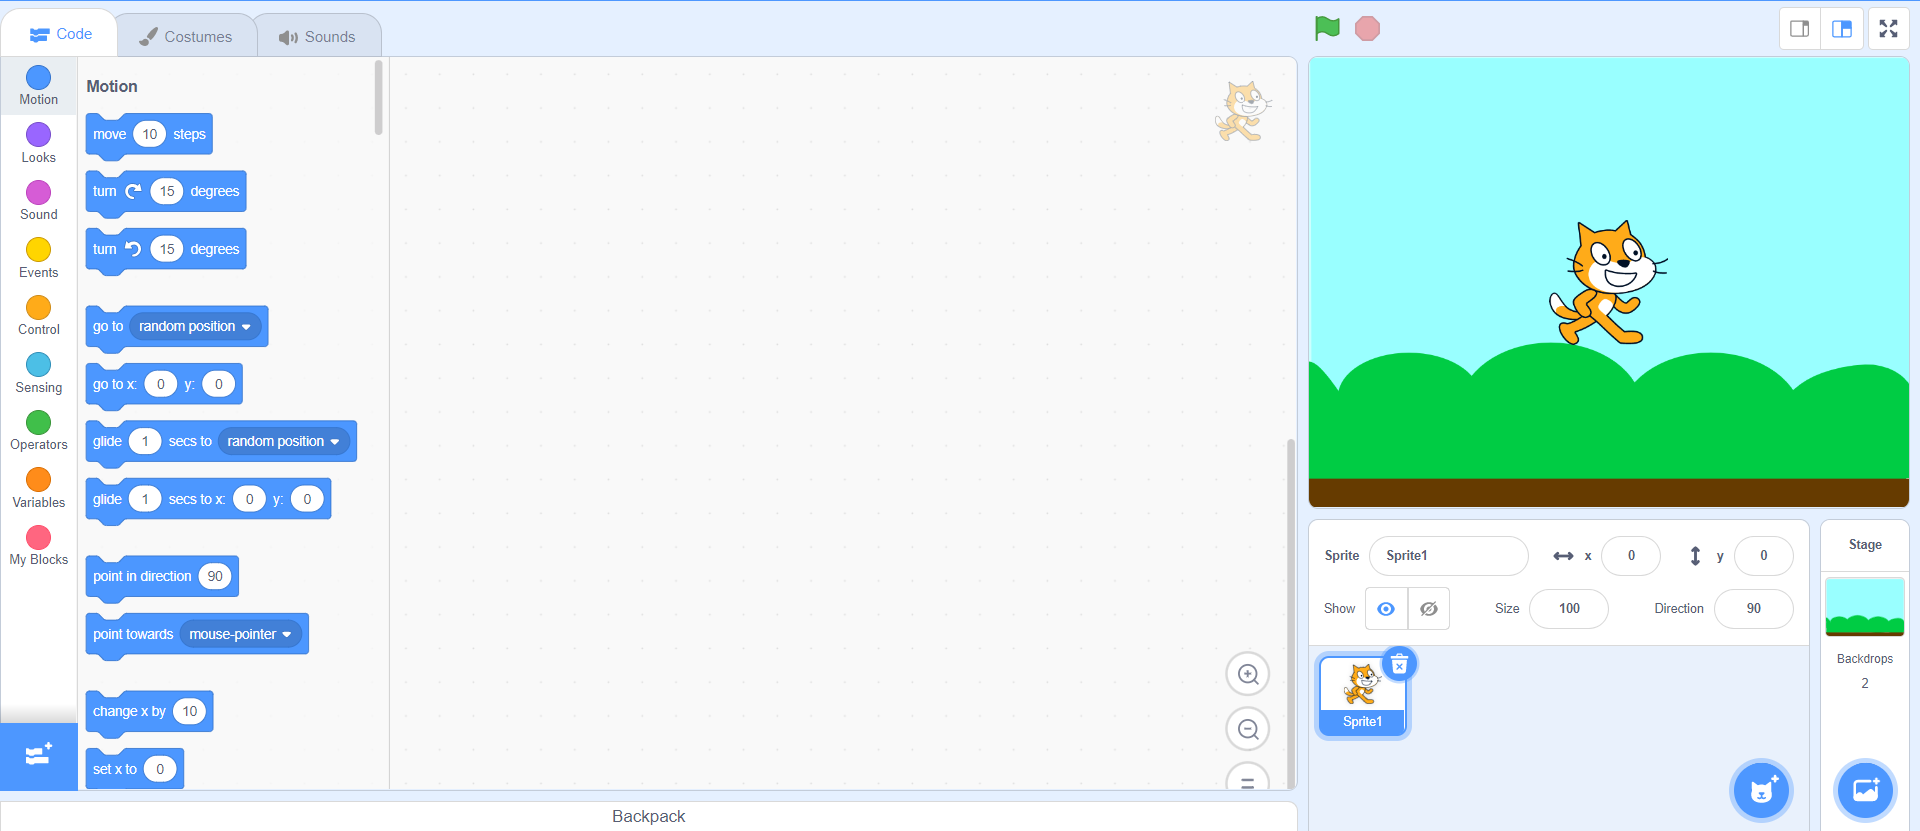
\includegraphics[width=1.0\linewidth,height=0.5\linewidth]{fig030002.png}
  \caption{Избор на подходящ фон за играта}
\label{fig030002}
\end{figure}

В тази гира, за да се направи състезателното трасе заедно със зелената финална линия, трябва фонът да бъде подобрен. За тази цел първо се избира опция Bacdrops.

\begin{figure}[H]
  \centering
  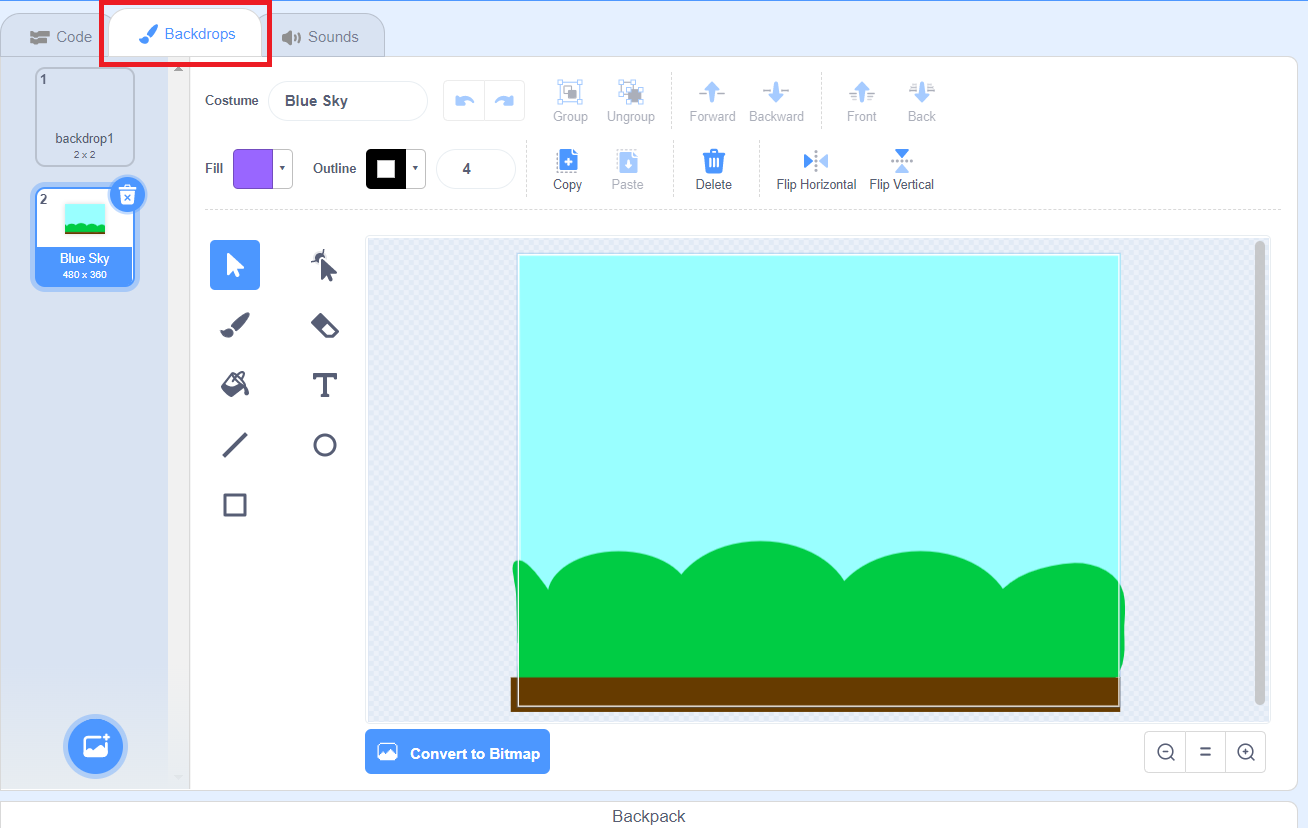
\includegraphics[width=1.0\linewidth,height=0.5\linewidth]{fig030003.png}
  \caption{Рисуване на допълнителни елементи върху фона}
\label{fig030003}
\end{figure}

С помощта на инструмента линия се добавя състезателното трасе. Ако се смени дебелината и цвета на линията може да бъде добавена и финалната линия.

\begin{figure}[H]
  \centering
  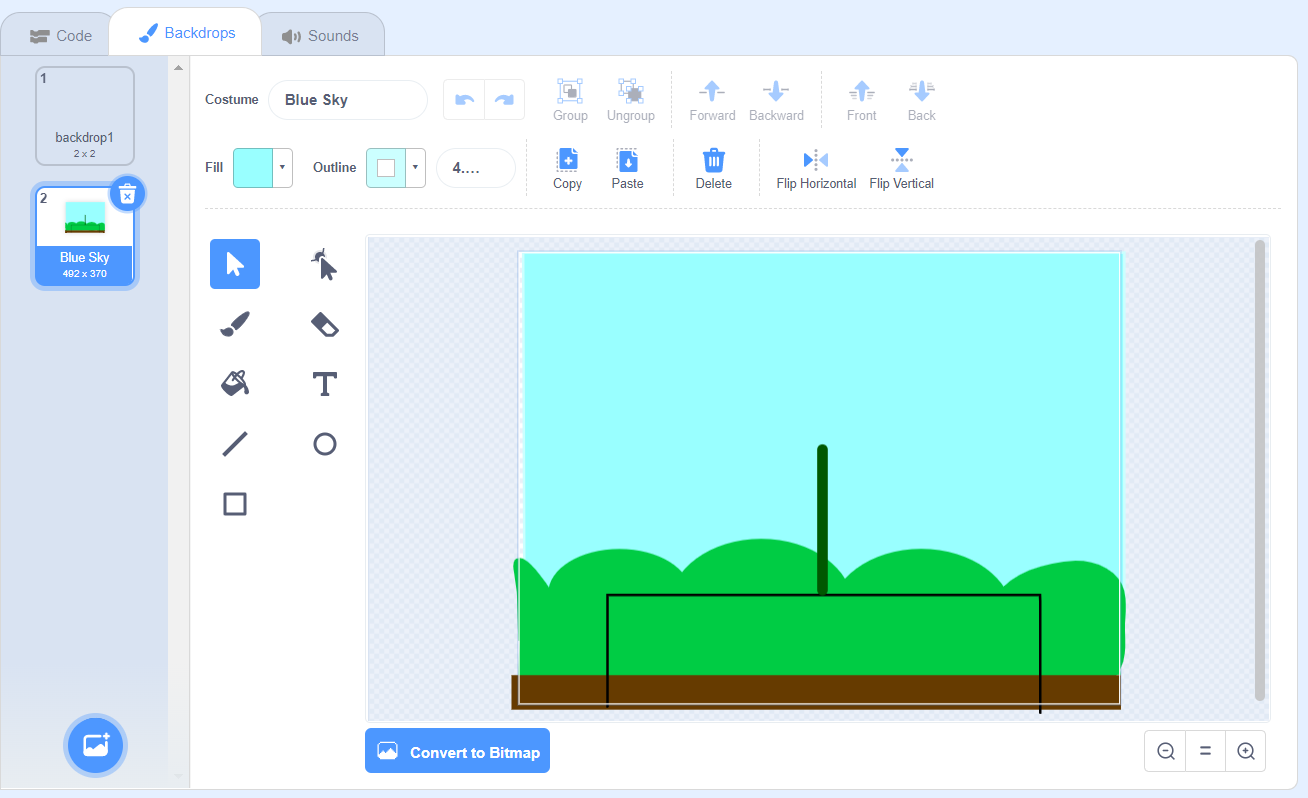
\includegraphics[width=1.0\linewidth,height=0.5\linewidth]{fig030004.png}
  \caption{Финален фон на играта}
\label{fig030004}
\end{figure}

Ако играта няма нужда от основния герой в Scratch котката, той може да бъде изтрит.

\begin{figure}[H]
  \centering
  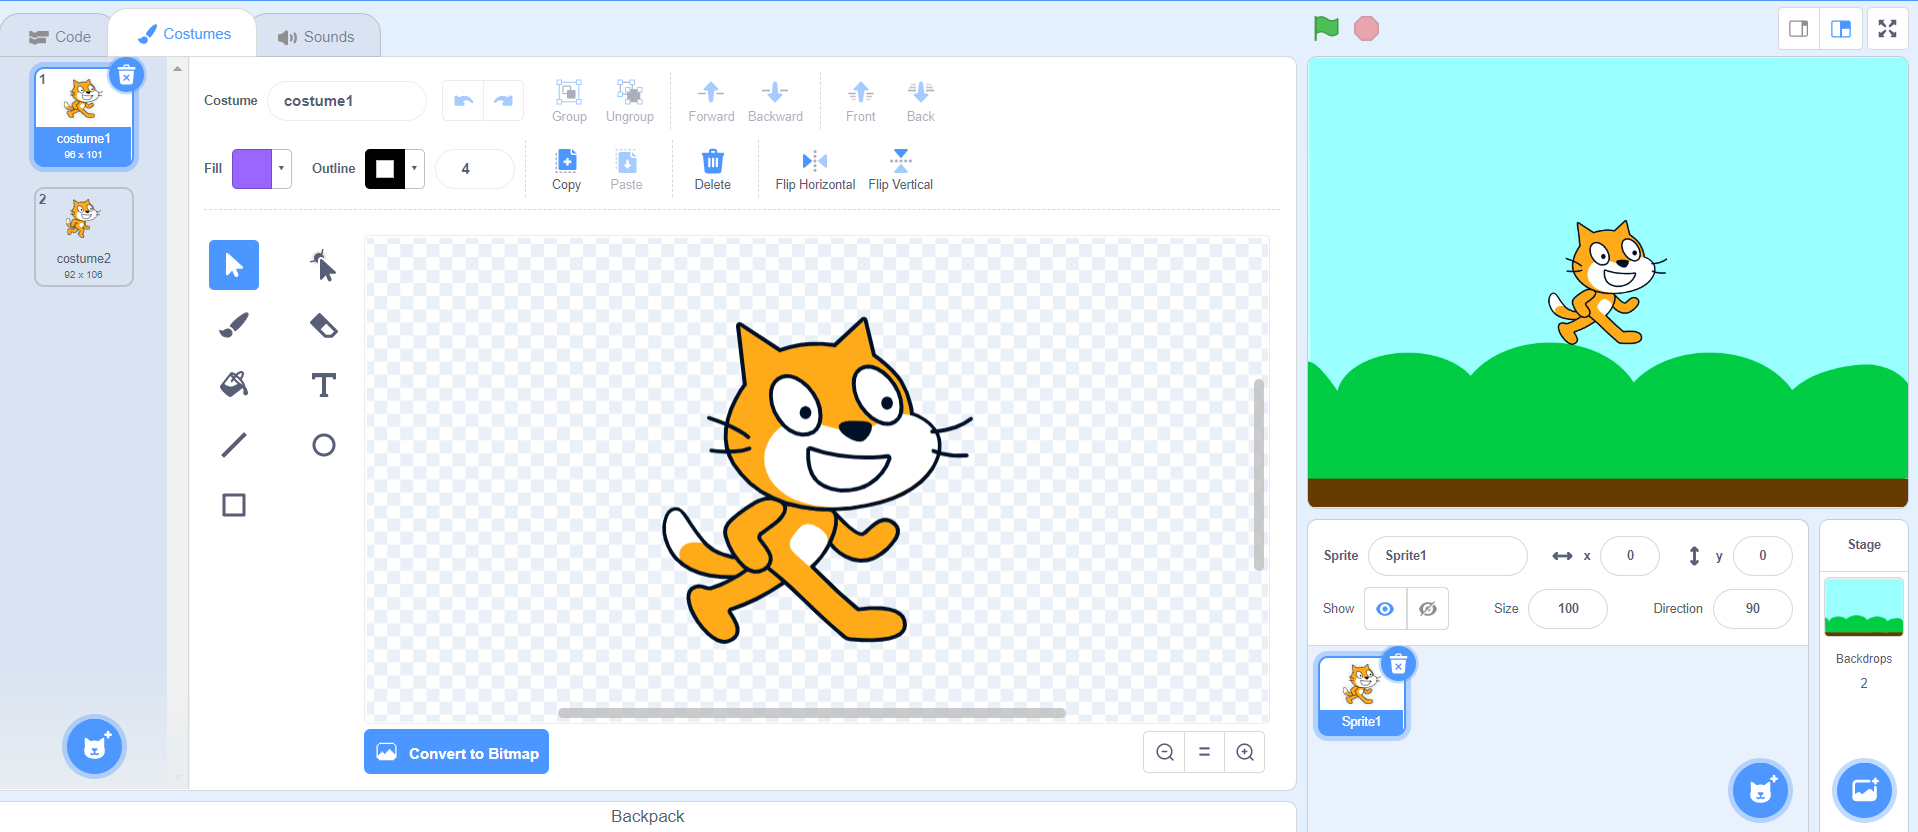
\includegraphics[width=1.0\linewidth,height=0.5\linewidth]{fig030005.png}
  \caption{Изтриване на основния герой}
\label{fig030005}
\end{figure}

Следва да бъдат добавени и героите към играта. В Scratch има налични много спрайтове. За целите на тази игра са необходими два - един, който е позициониран в ляво и друг - в дясно (Фиг. \ref{fig030006}). Чрез свойствата Size и Direction се променя размерът и посоката на героя.

\begin{figure}[H]
  \centering
  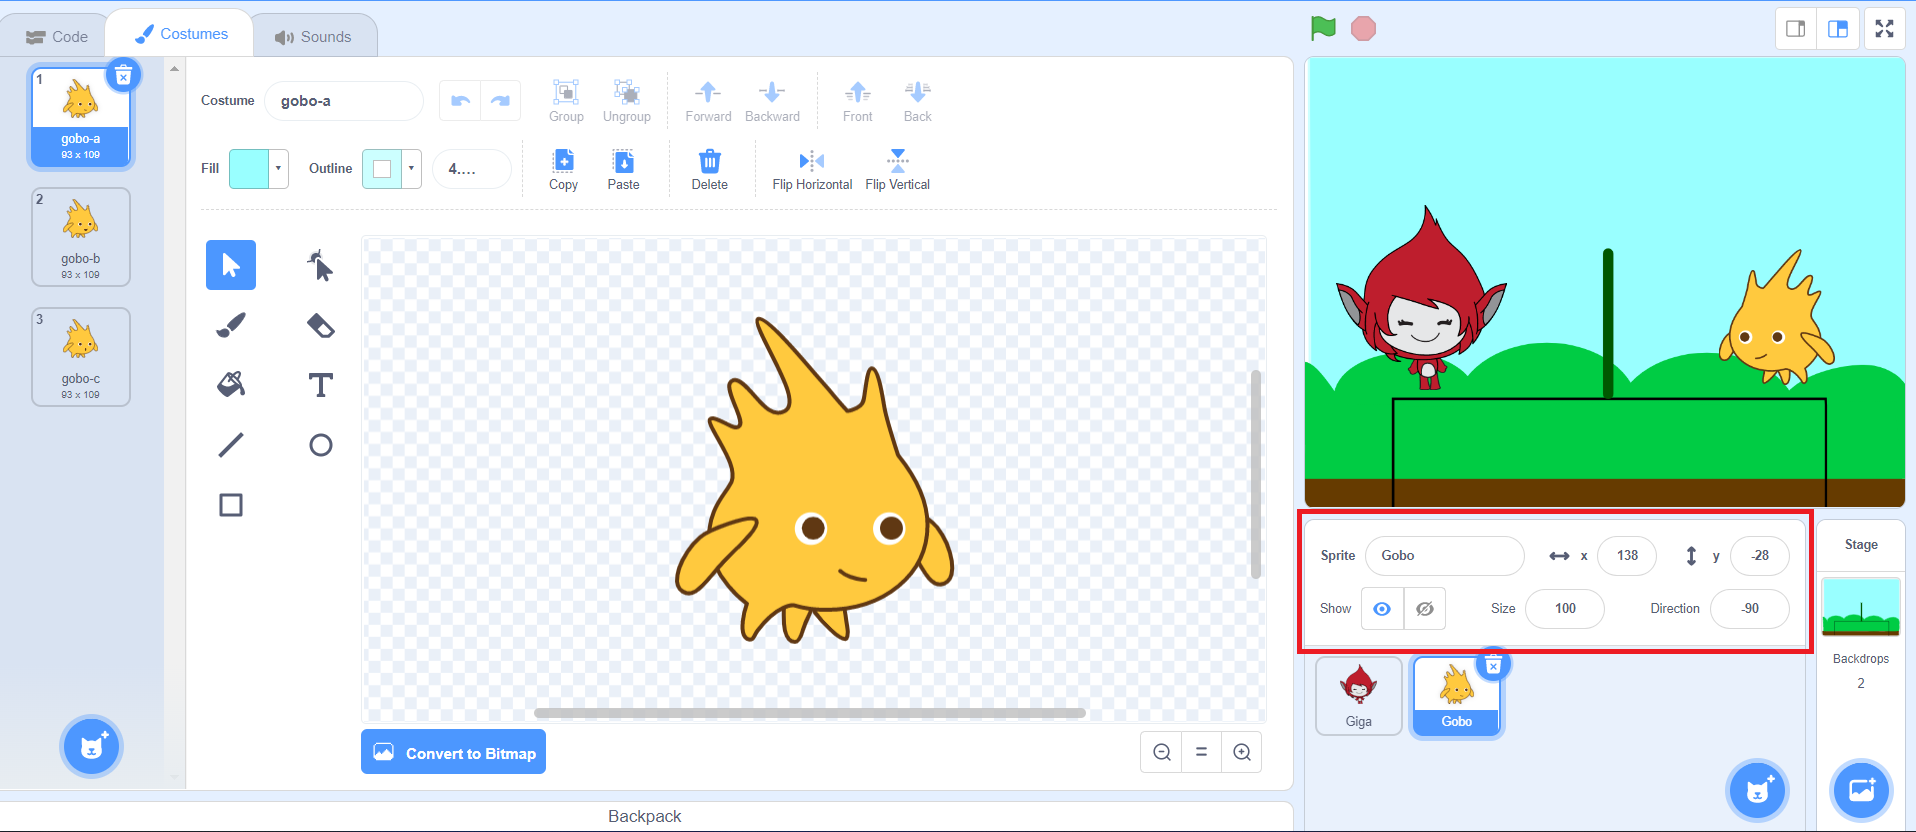
\includegraphics[width=1.0\linewidth,height=0.5\linewidth]{fig030006.png}
  \caption{Герои в играта}
\label{fig030006}
\end{figure}

Освен тези два спрайта са необходими и още два, които са бутоните, върху които играчите трябва да кликат. Те се намират отново в секция Sprite. В тази игра бутоните трябва да бъдат различен цвят, за да се различават. За да се промени цвета на бутон, то трябва да се промени неговия костюм .

\begin{figure}[H]
  \centering
  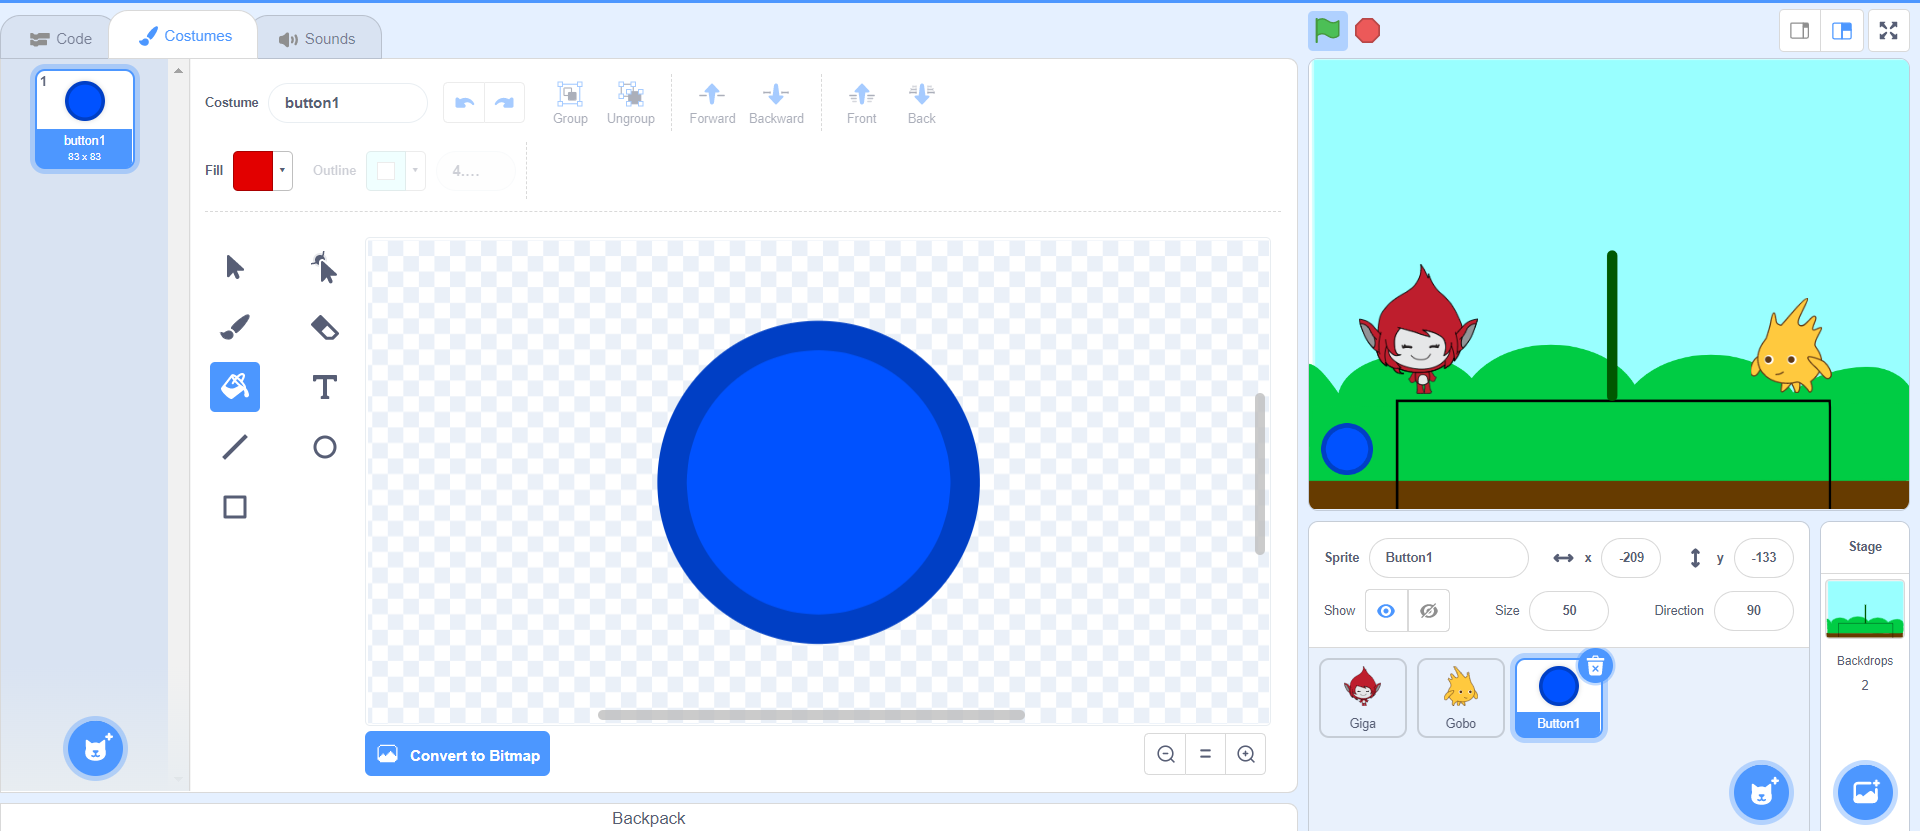
\includegraphics[width=1.0\linewidth,height=0.5\linewidth]{fig030007.png}
  \caption{Син бутон}
\label{fig030007}
\end{figure}

С помощта на инструмента Fill се сменя цвета на бутона (Фиг. \ref{fig030008}). Същото може да се направи и за червения бутон. Отново чрез свойството Size може да промени размерът на този спрайт.

\begin{figure}[H]
  \centering
  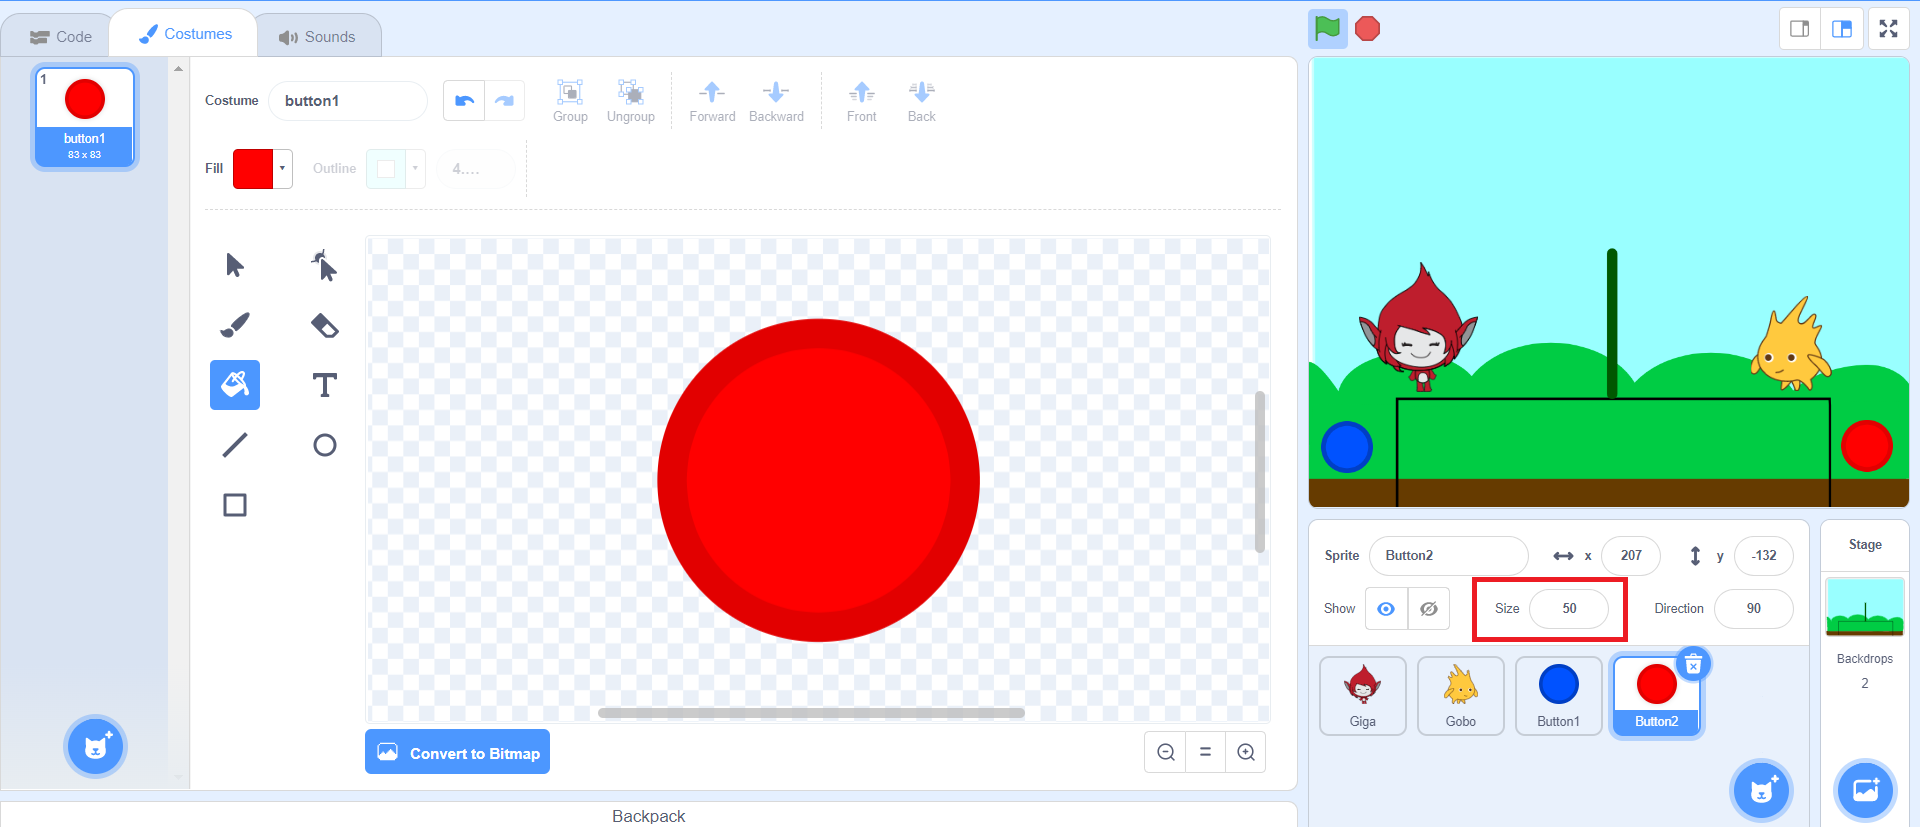
\includegraphics[width=1.0\linewidth,height=0.5\linewidth]{fig030008.png}
  \caption{Червен бутон}
\label{fig030008}
\end{figure}

\section{Програмиране на синия бутон}
Когато играчът кликне върху синия бутон, той трябва да изпрати съобщение "blue". Първото начално блокче, което трябва да се постави е когато този спрайт бъде кликнат.

\begin{figure}[H]
  \centering
  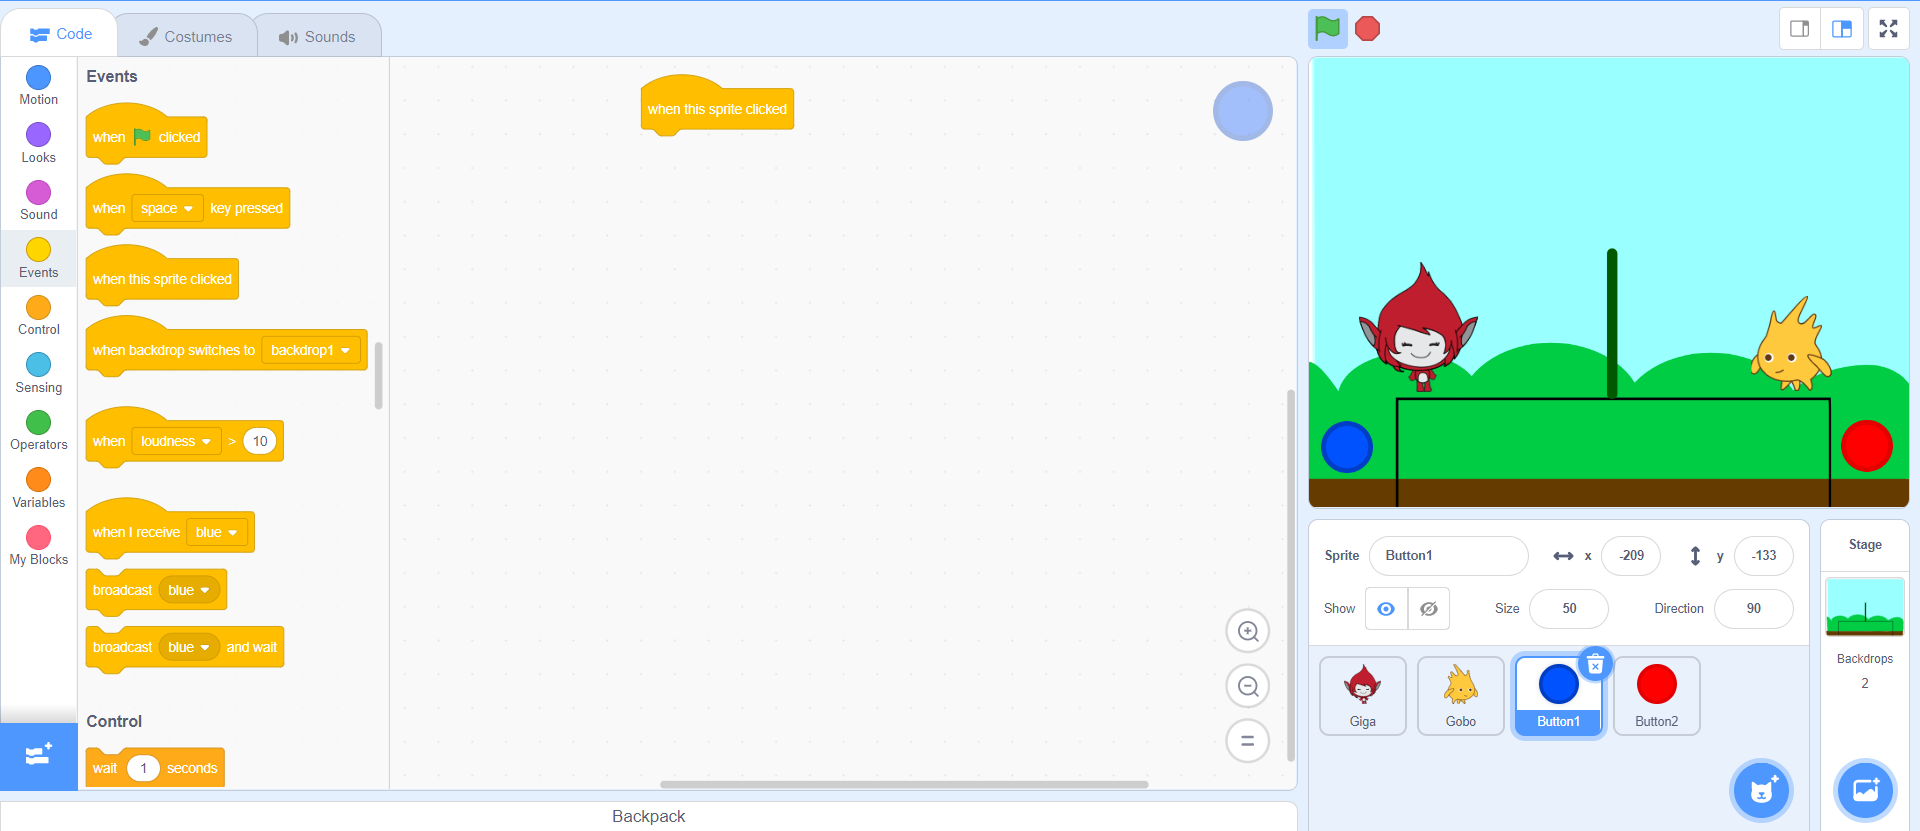
\includegraphics[width=1.0\linewidth,height=0.5\linewidth]{fig030009.png}
  \caption{Когато героят е кликнат}
\label{fig030009}
\end{figure}

Следва героят да изпрати съобщение "blue". От тъмно оранжевата група инструкцията за разпространение на съобщение. Съобщението, което трябва да разпространи е "blue".

\begin{figure}[H]
  \centering
  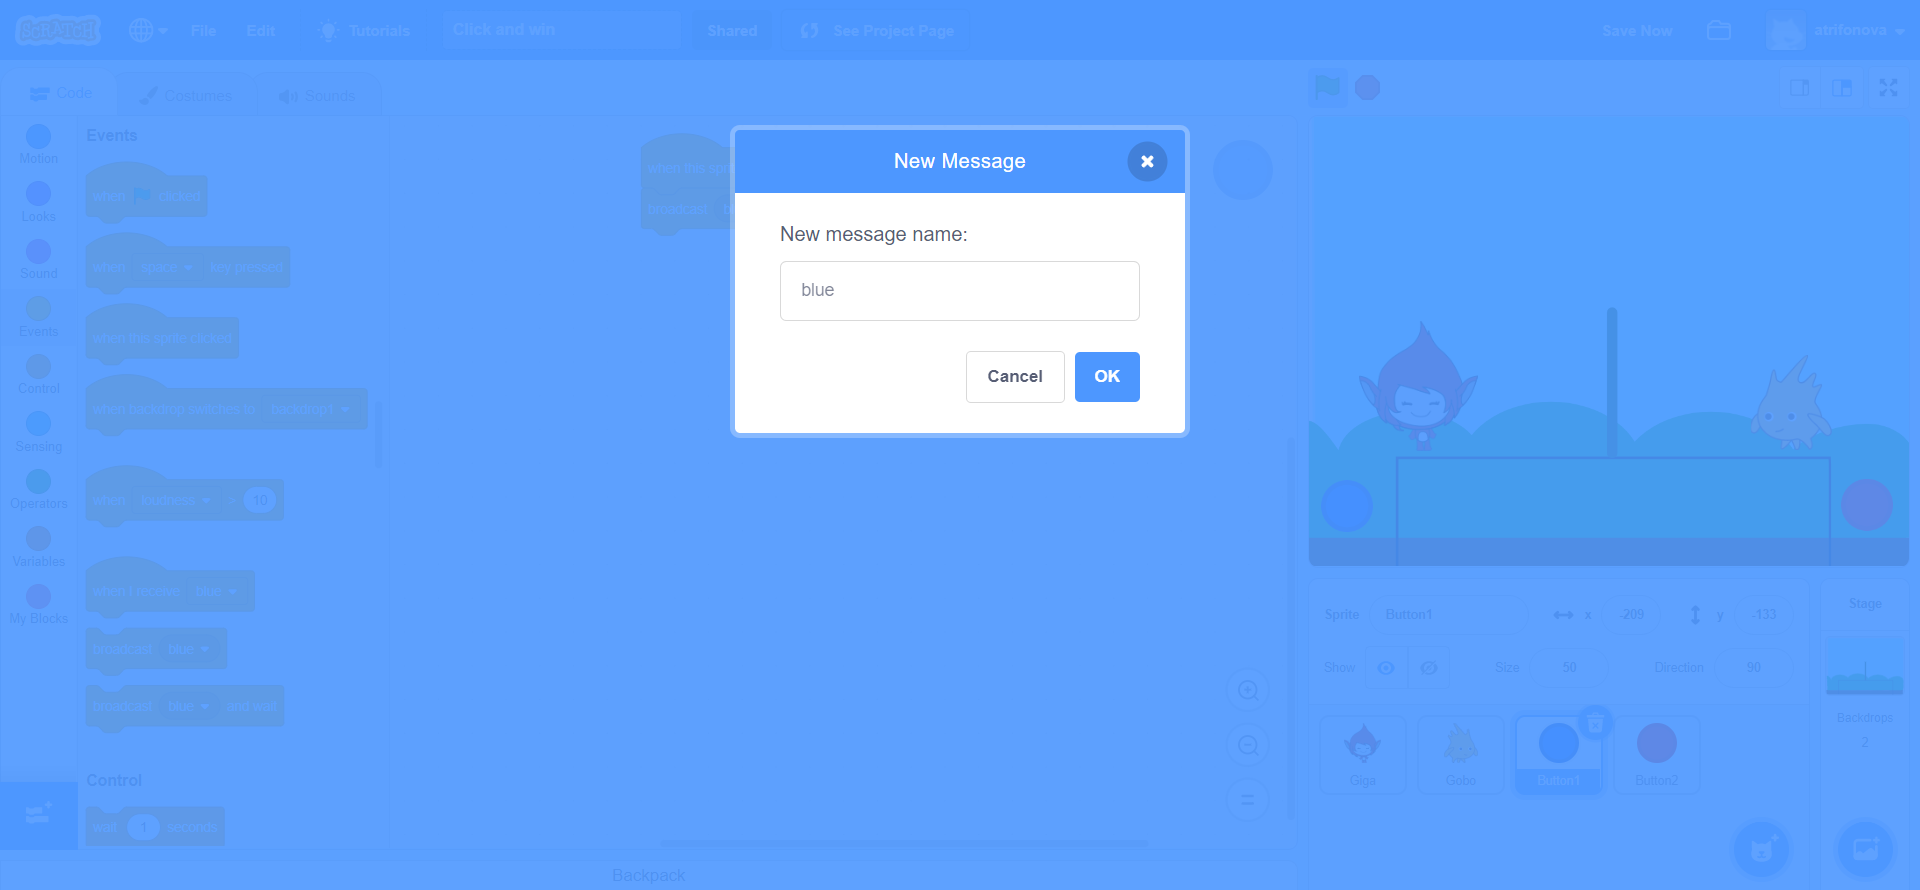
\includegraphics[width=1.0\linewidth,height=0.5\linewidth]{fig030010.png}
  \caption{Изпращане на съобщение}
\label{fig030010}
\end{figure}

Кодът на този герой изглежда по следния начин:

\begin{figure}[H]
  \centering
  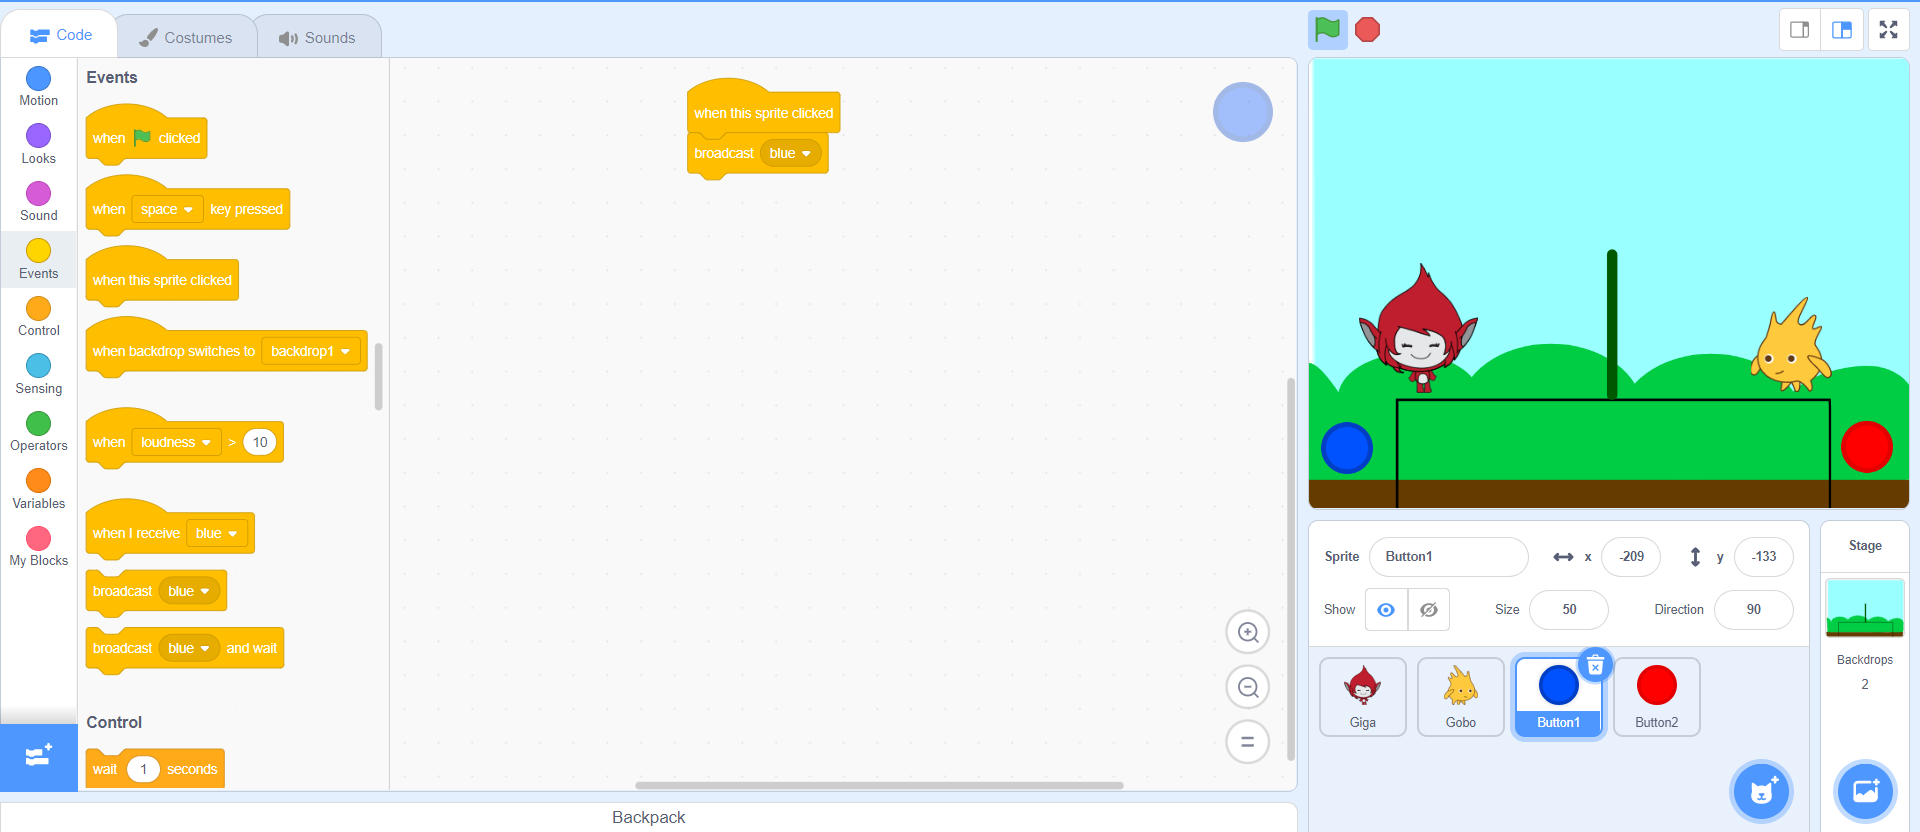
\includegraphics[width=1.0\linewidth,height=0.5\linewidth]{fig030011.png}
  \caption{Целият код на синия бутон}
\label{fig030011}
\end{figure}

\section{Програмиране на червения бутон}
Когато играчът кликне върху червения бутон, аналогично на синия, той трябва да изпрати съобщение "red". Кодът на червения бутон е следния:

\begin{figure}[H]
  \centering
  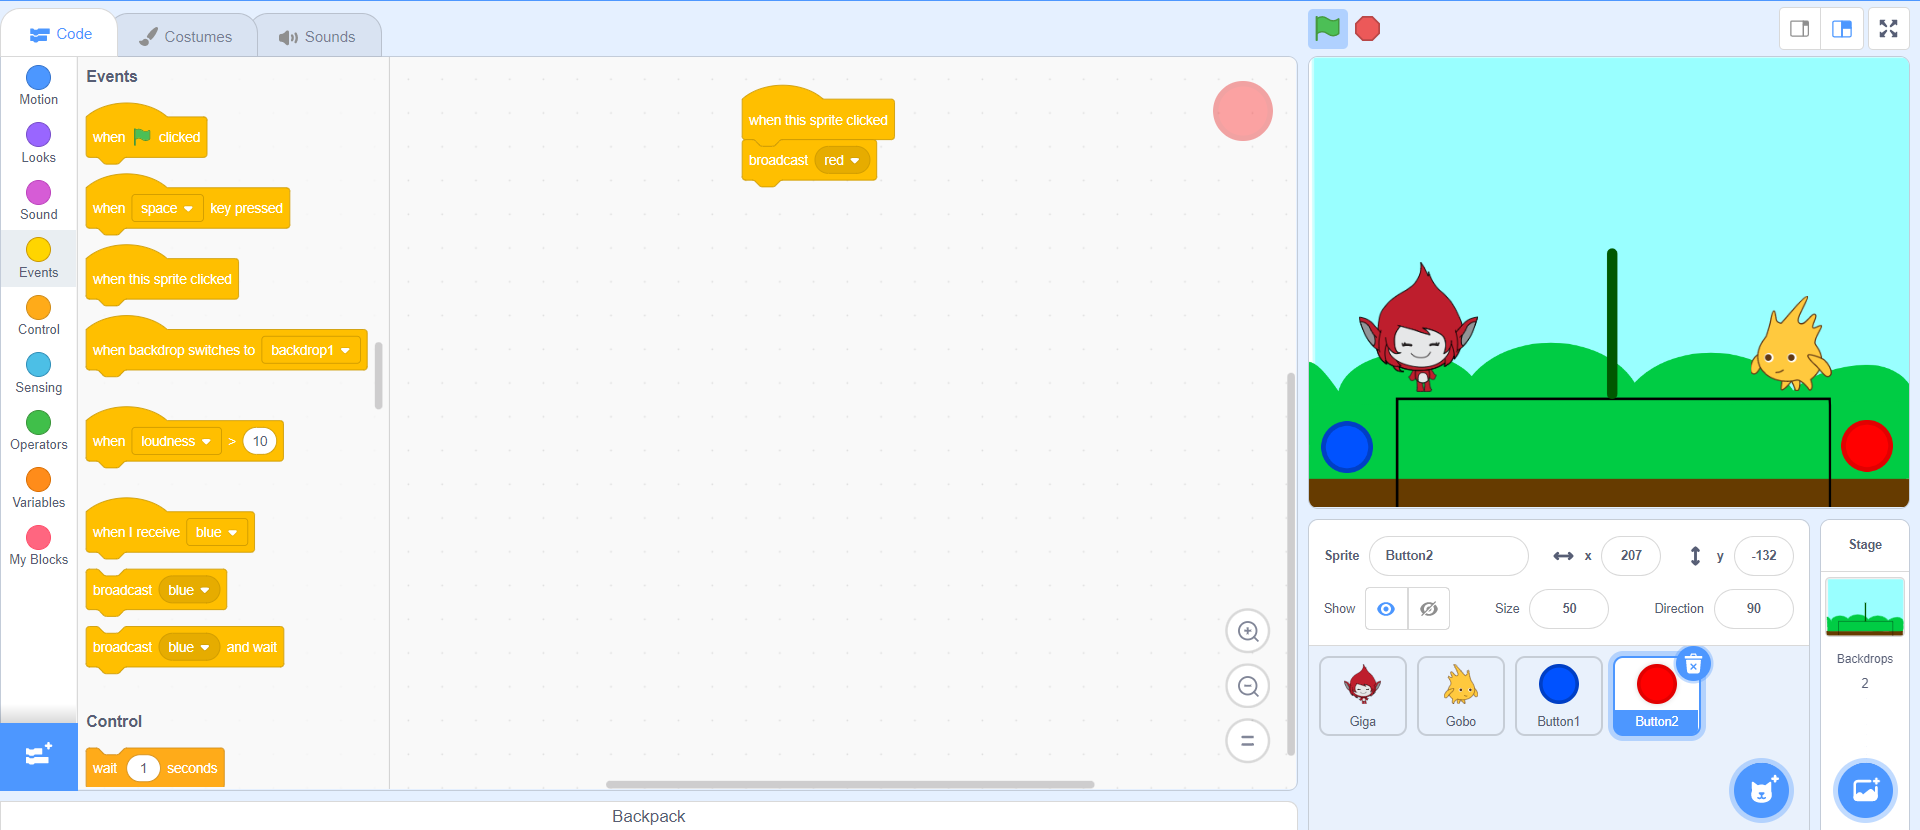
\includegraphics[width=1.0\linewidth,height=0.5\linewidth]{fig030012.png}
  \caption{Целият код на червения бутон}
\label{fig030012}
\end{figure}

До този момент програмата се състои в това, когато играчът натисне синия или червения бутон, те да изпращат съответните съобщения.

\section{Програмиране героите да се движат}
Инструкциите на синия бутон са, че той изпраща съобщение. Левият герой трябва да се абонира да получи съобщението.

\begin{figure}[H]
  \centering
  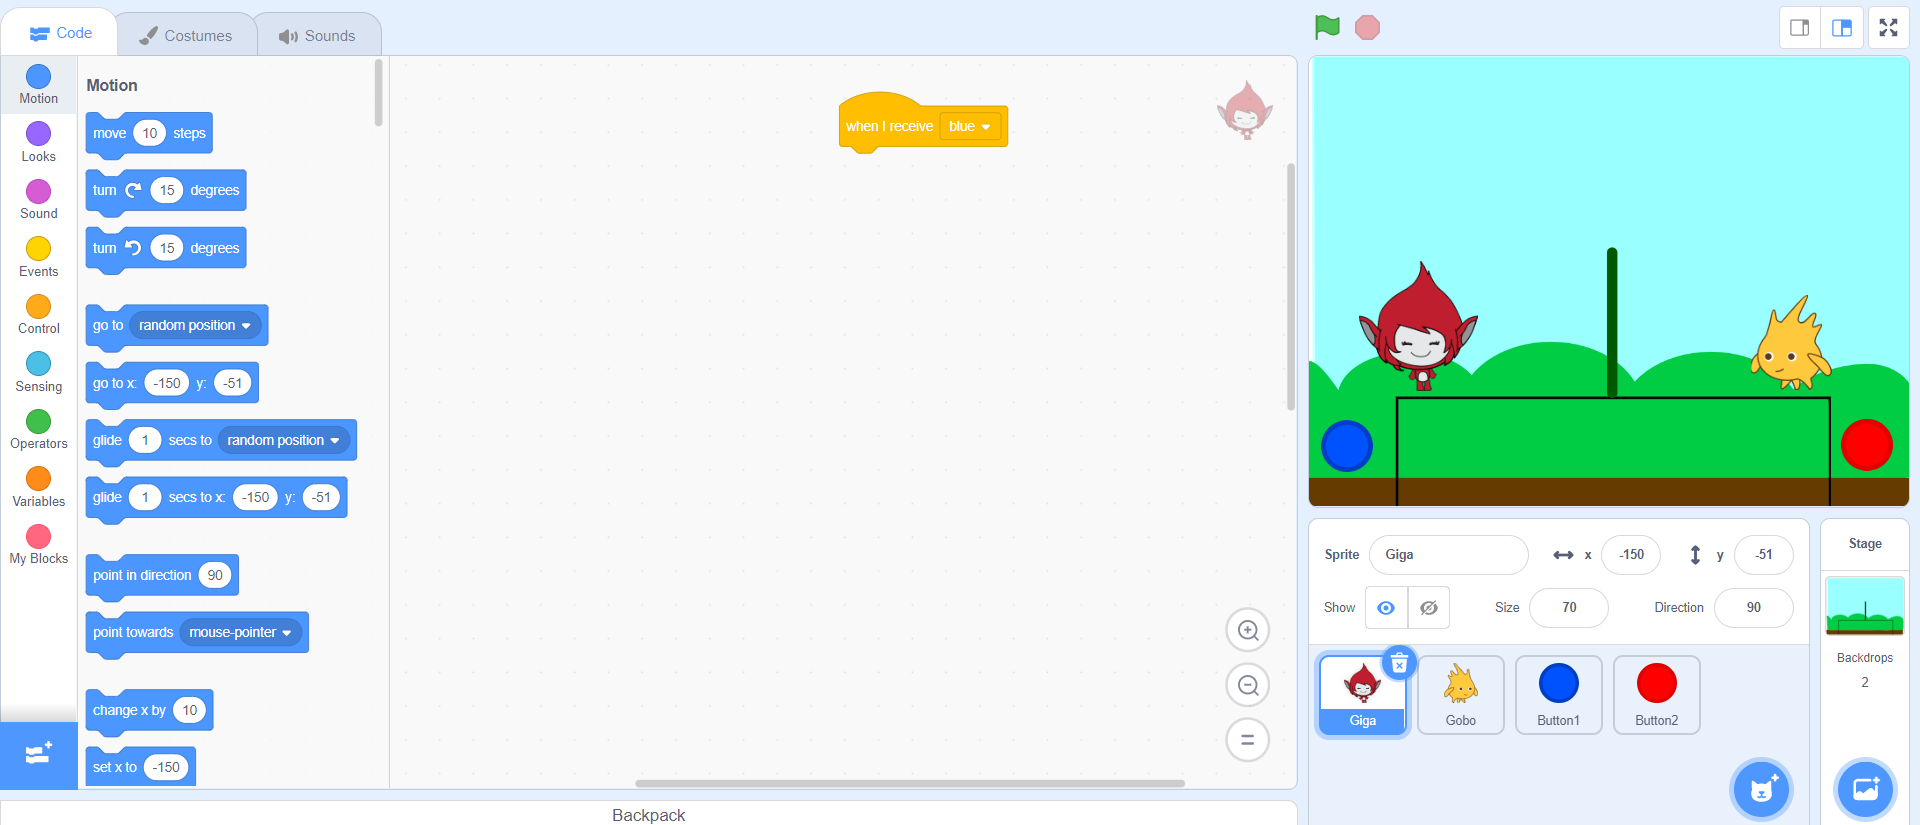
\includegraphics[width=1.0\linewidth,height=0.5\linewidth]{fig030013.png}
  \caption{Абониране за съобщението от синия бутон}
\label{fig030013}
\end{figure}

Героят трябва да се премести надясно към зелената финална линия, което означава, че трябва да се промени x координатата, като се увеличи с 3 стъпки.

\begin{figure}[H]
  \centering
  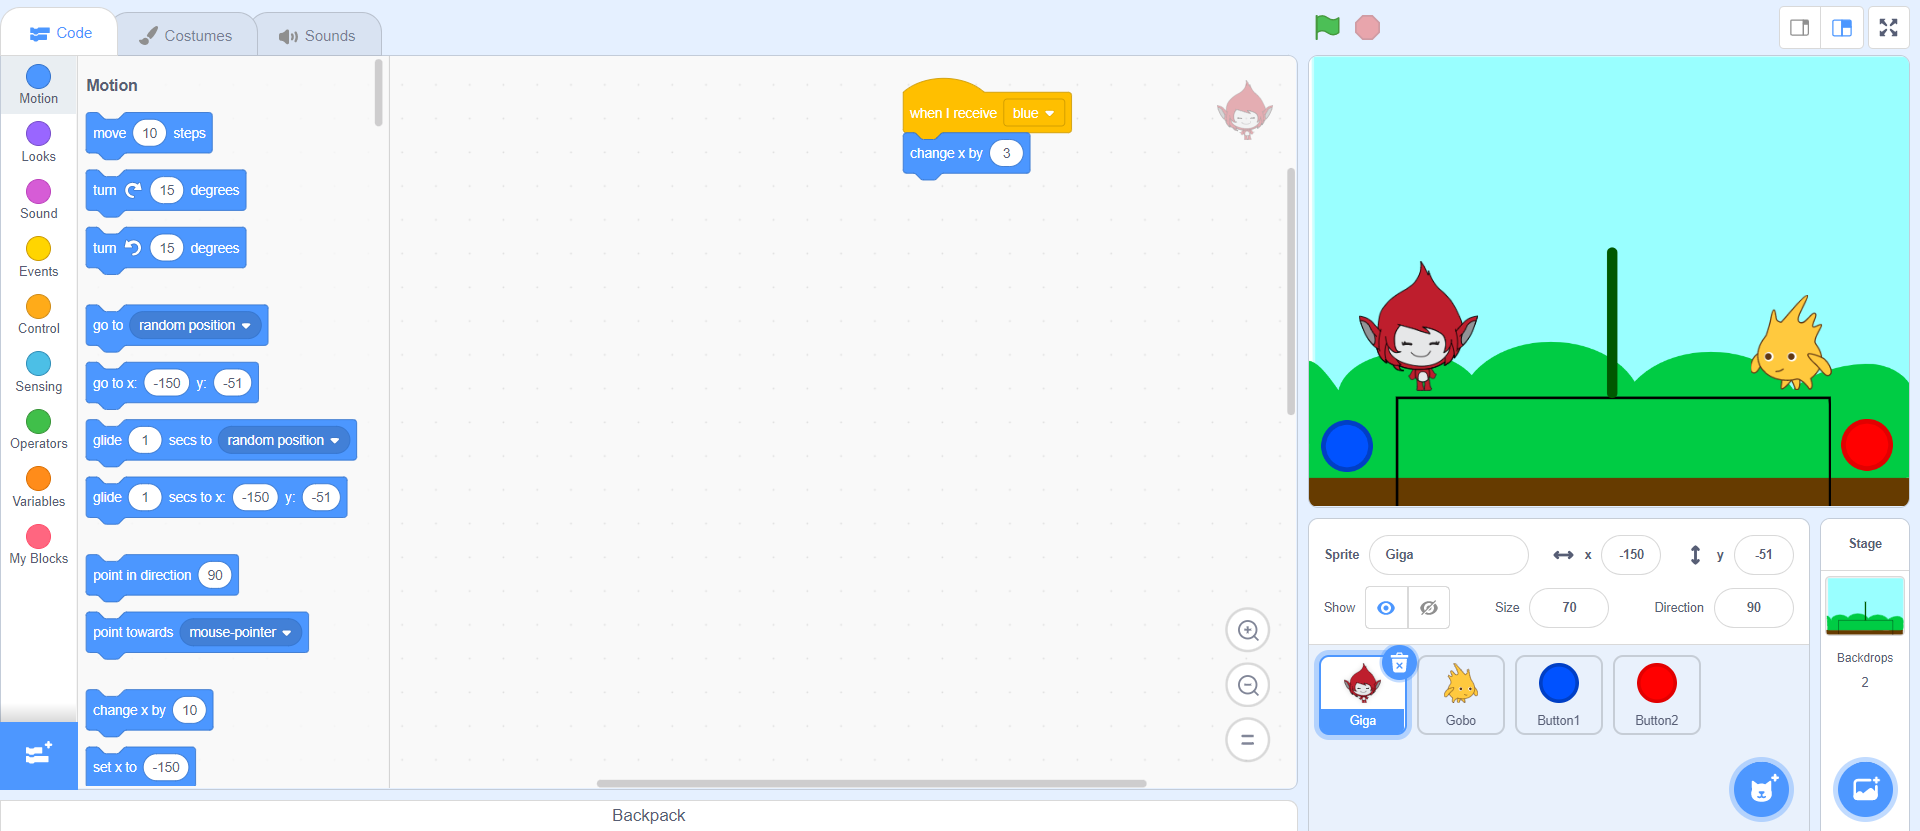
\includegraphics[width=1.0\linewidth,height=0.5\linewidth]{fig030014.png}
  \caption{Движение на героя надясно}
\label{fig030014}
\end{figure}

Инструкциите за другият герой е аналогичен. Основните разлики са две:
- съобщението, за което този герой се абонира е изпратено от червения бутон
- героят трябва да се движи наляво към зелената финална линия, което означава, че трябва да се промени x координатата, като се намали с 3 стъпки

\begin{figure}[H]
  \centering
  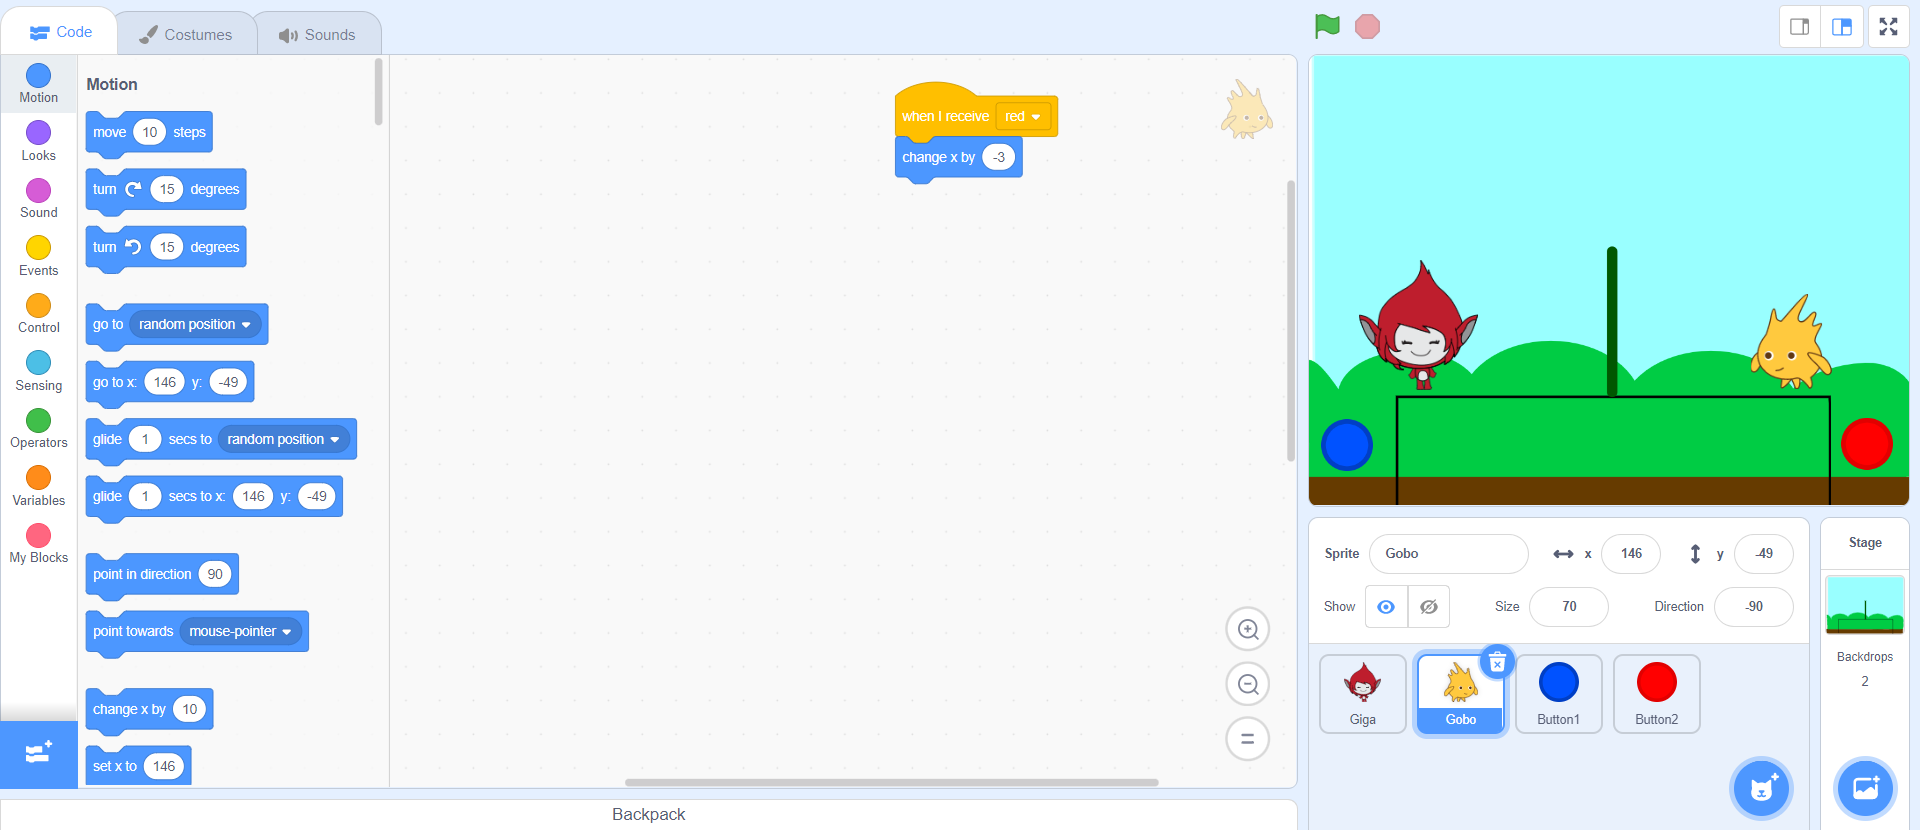
\includegraphics[width=1.0\linewidth,height=0.5\linewidth]{fig030015.png}
  \caption{Движение на героя наляво}
\label{fig030015}
\end{figure}

\section{Програмиране победителя}
За да се завърши играта остава да се направи проверка кой от героите е достигнал зелената финална линия.

В десния герой първата инструкция, която трябва да се добави е началната за начало на играта. Във всеки един момент на играта трябва да се проверява дали героят е достигнал до финалната линия. Поради тази причина трябва да се добави инструкция за цикъл завинаги.

\begin{figure}[H]
  \centering
  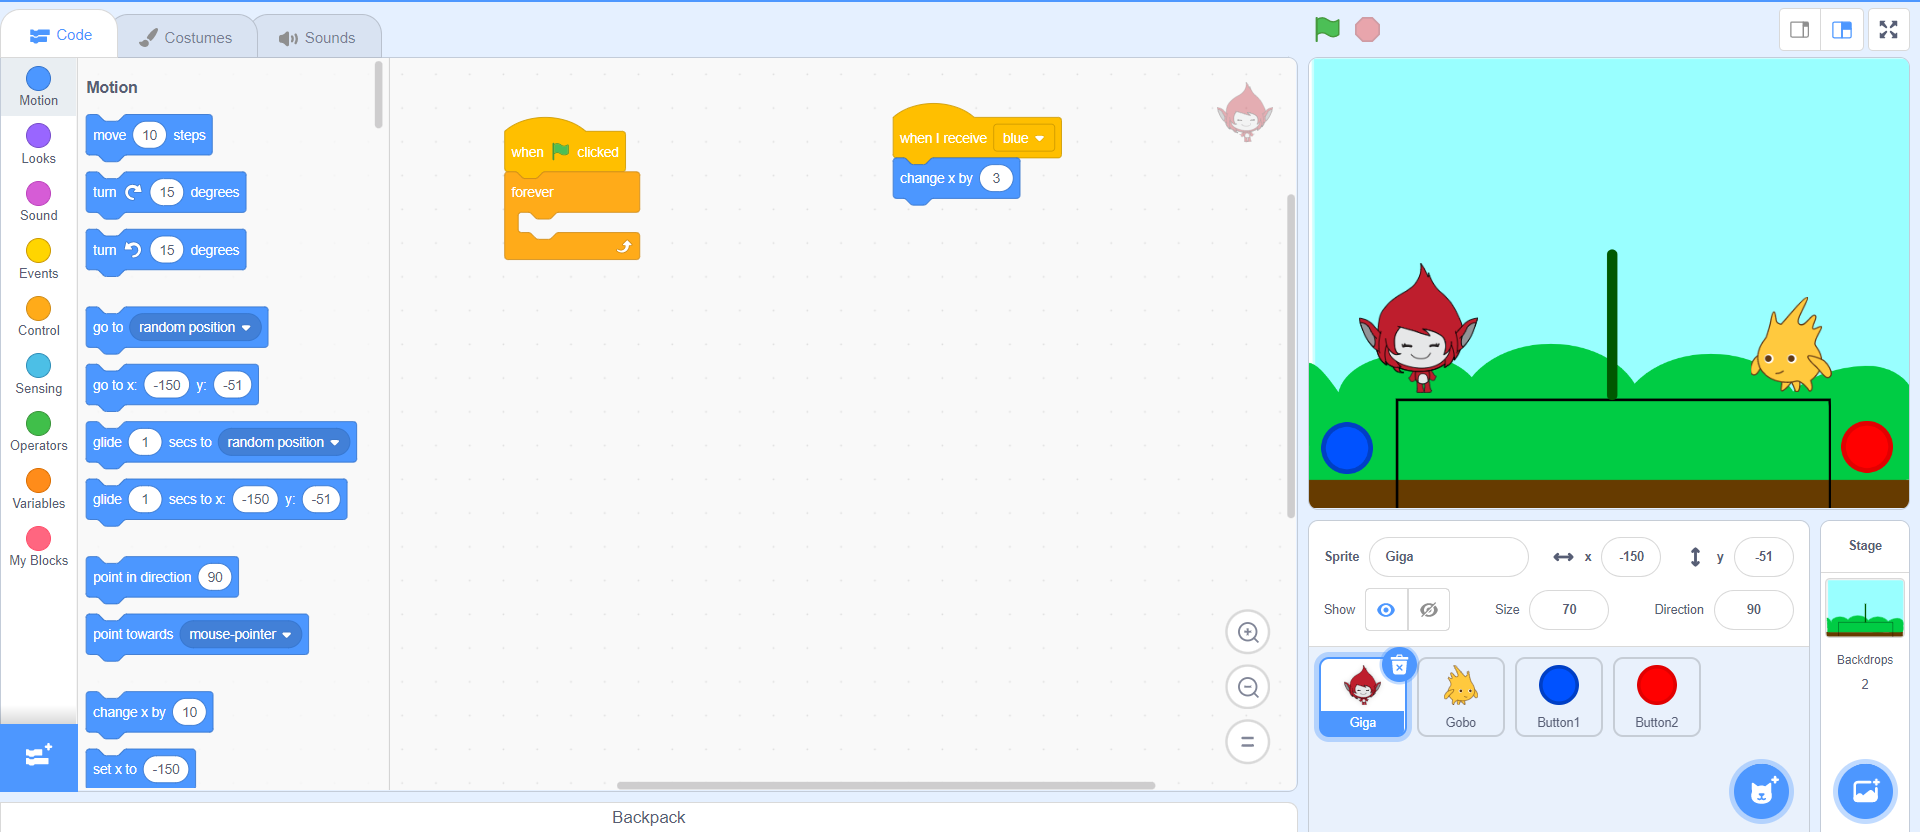
\includegraphics[width=1.0\linewidth,height=0.5\linewidth]{fig030016.png}
  \caption{Цикъл завинаги}
\label{fig030016}
\end{figure}

Вътре в тялото на цикъла следва да се направи проверката, за това дали героят е докоснал финалната линия.

\begin{figure}[H]
  \centering
  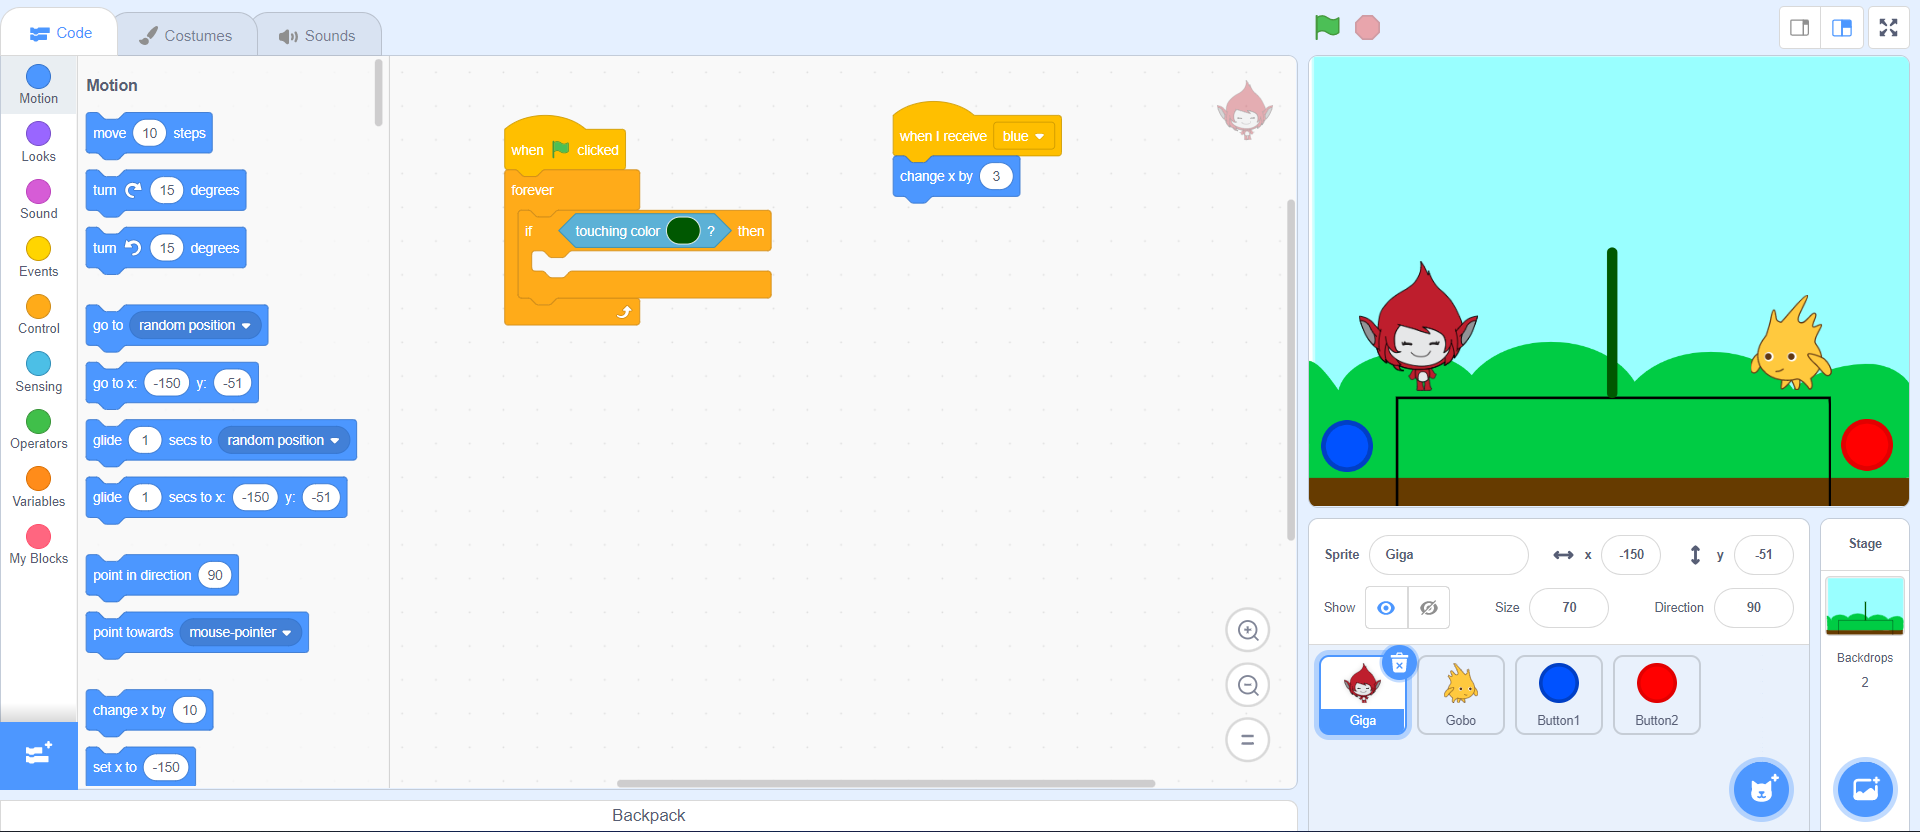
\includegraphics[width=1.0\linewidth,height=0.5\linewidth]{fig030017.png}
  \caption{Проверка дали героят е достигнал финал}
\label{fig030017}
\end{figure}

За да се избере същия зелен цвят, какъвто е на финалната линия, трябва да се използва инструментът пипетка.

\begin{figure}[H]
  \centering
  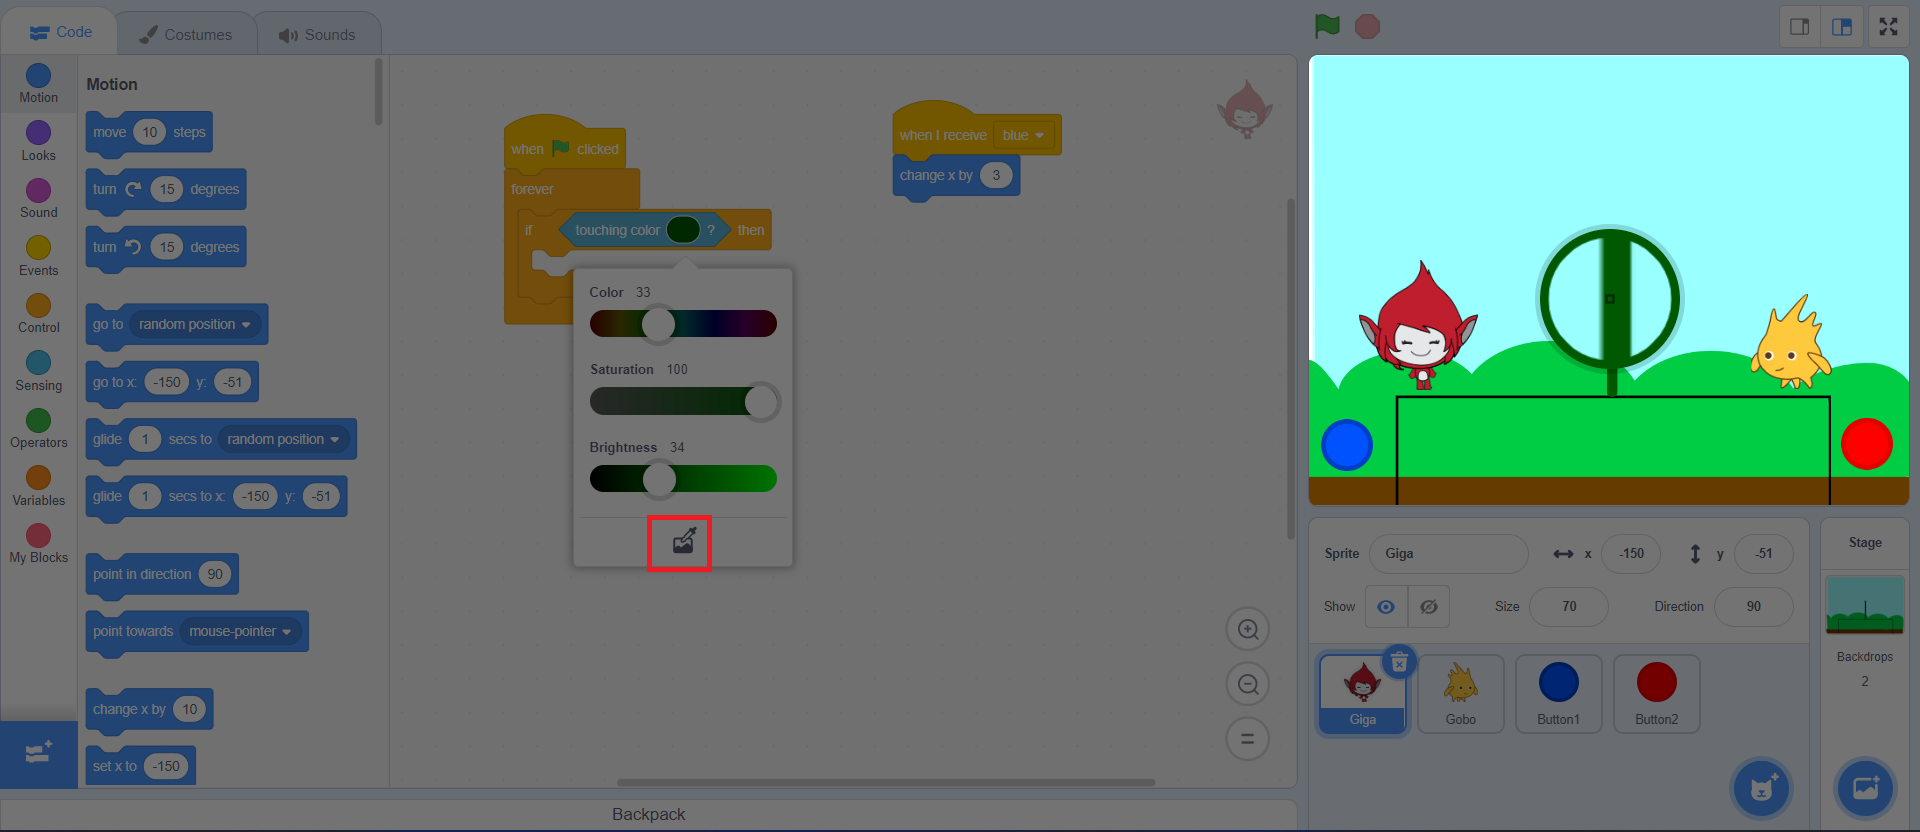
\includegraphics[width=1.0\linewidth,height=0.5\linewidth]{fig030018.png}
  \caption{Избор на цвят}
\label{fig030018}
\end{figure}

Инструкциите, които се намират вътре в условието ще се изпълнят, когато героят победи. Тогава той трябва да уголеми размера си и да изпише съобщение "Победих!".

\begin{figure}[H]
  \centering
  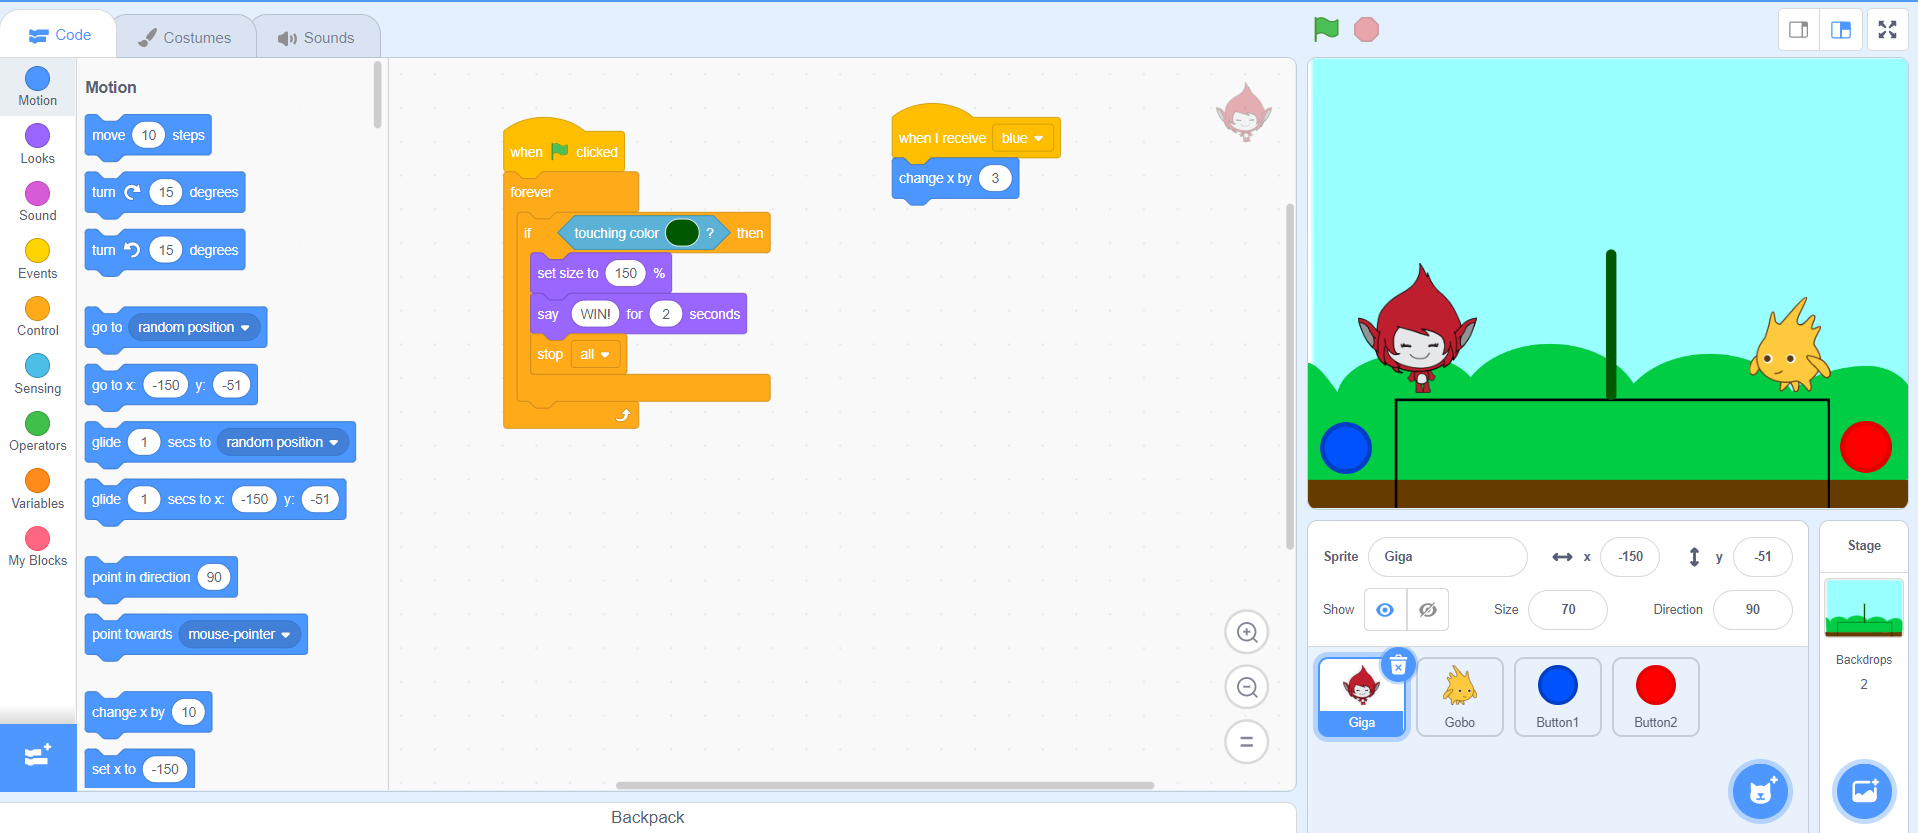
\includegraphics[width=1.0\linewidth,height=0.5\linewidth]{fig030019.png}
  \caption{Инструкциите за победа}
\label{fig030019}
\end{figure}

Последното подобрение, което трябва да се направи, за да се завърши този герой е да бъде поставен в начална позиция всеки път, когато играта започне. В синята секция се намира инструкцията, която казва къде да бъде позициониран героят.

\begin{figure}[H]
  \centering
  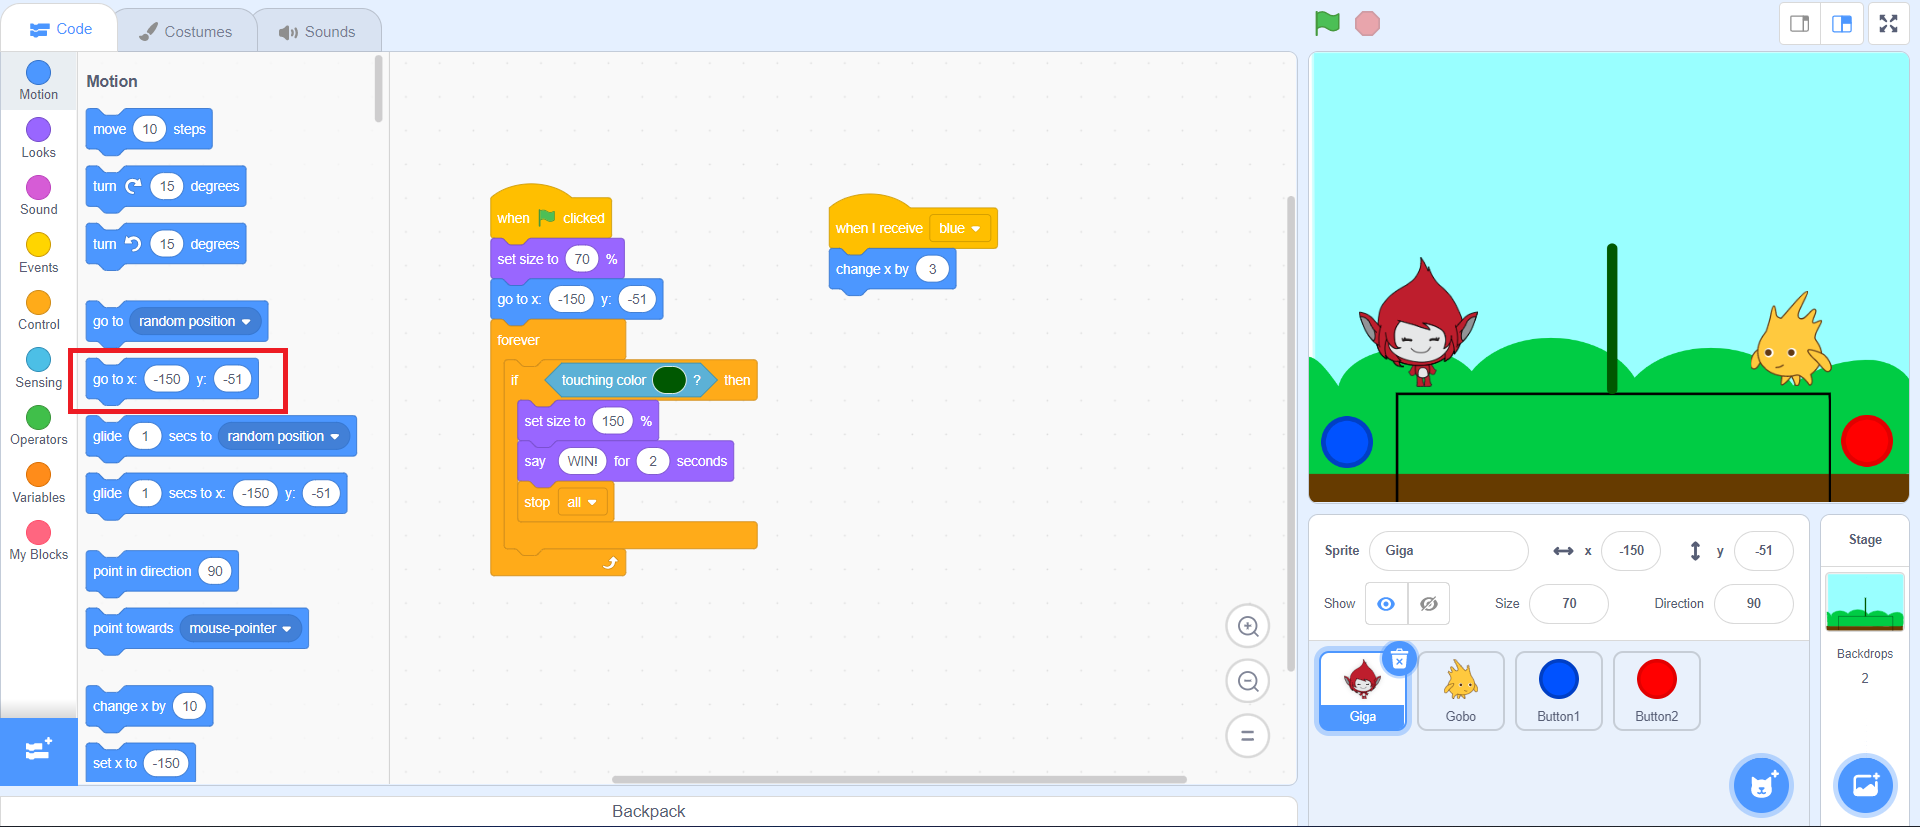
\includegraphics[width=1.0\linewidth,height=0.5\linewidth]{fig030020.png}
  \caption{Инструкцията за позициониране на героя}
\label{fig030020}
\end{figure}

Финалния код на този герой е:

\begin{figure}[H]
  \centering
  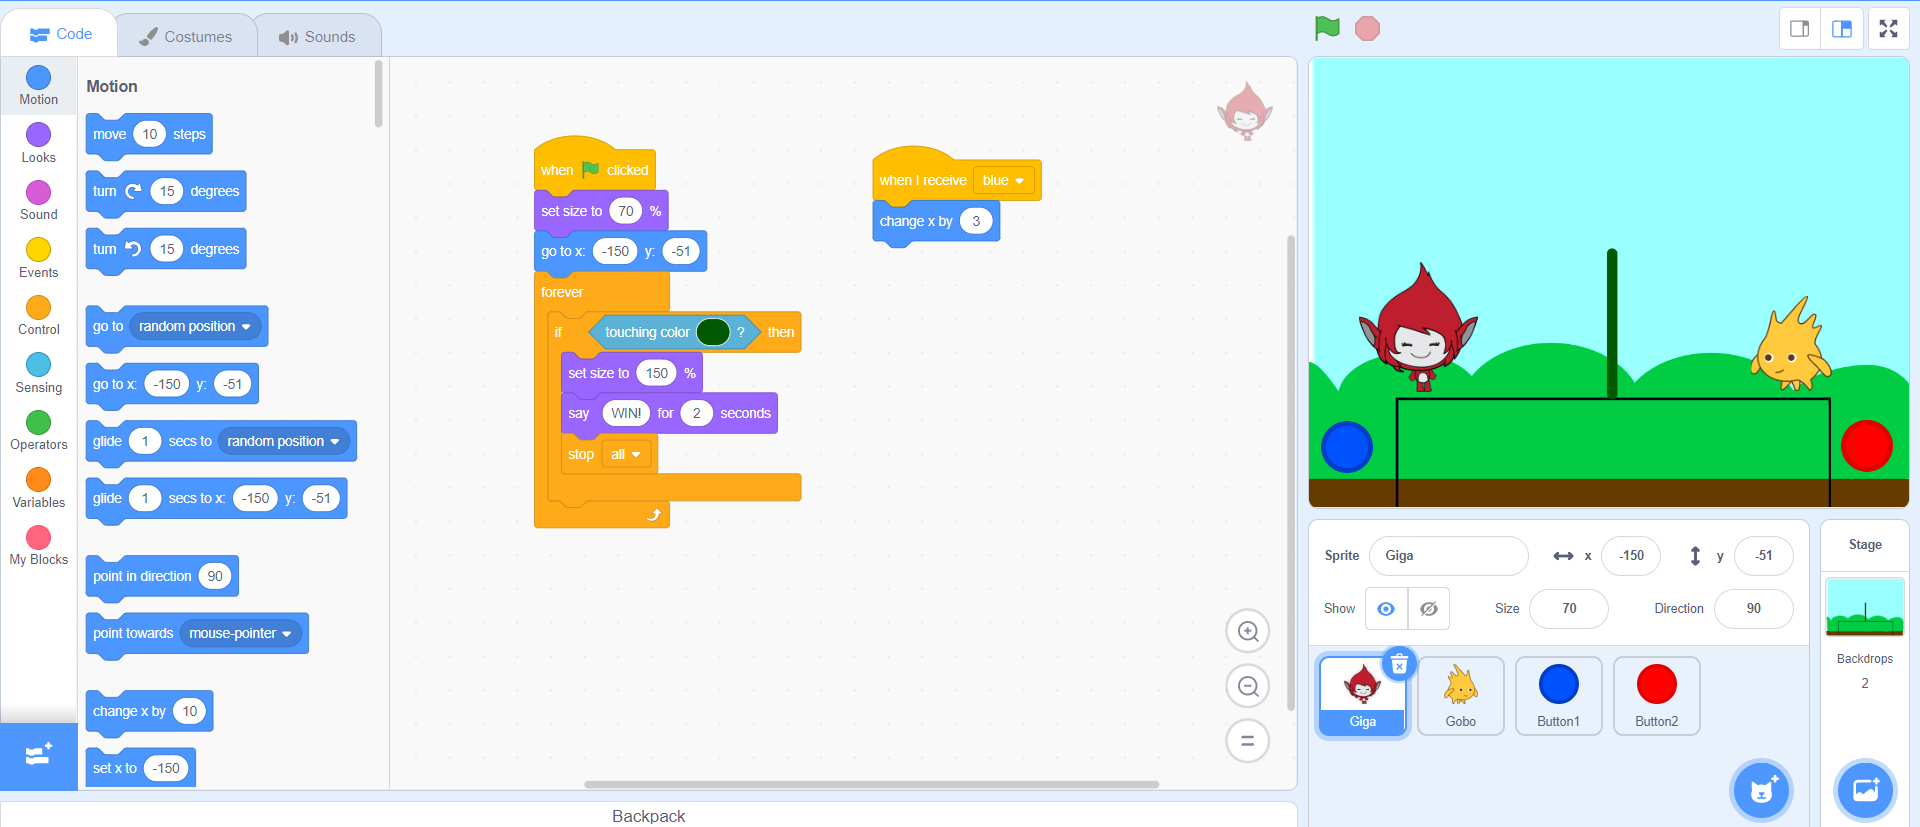
\includegraphics[width=1.0\linewidth,height=0.5\linewidth]{fig030021.png}
  \caption{Финален код на левия герой}
\label{fig030021}
\end{figure}

След като този герой е готов, остава да се добавят и инструкциите за победа и на другия герой. Кодът е аналогичен. Единствената разлика е в началните координати.

\begin{figure}[H]
  \centering
  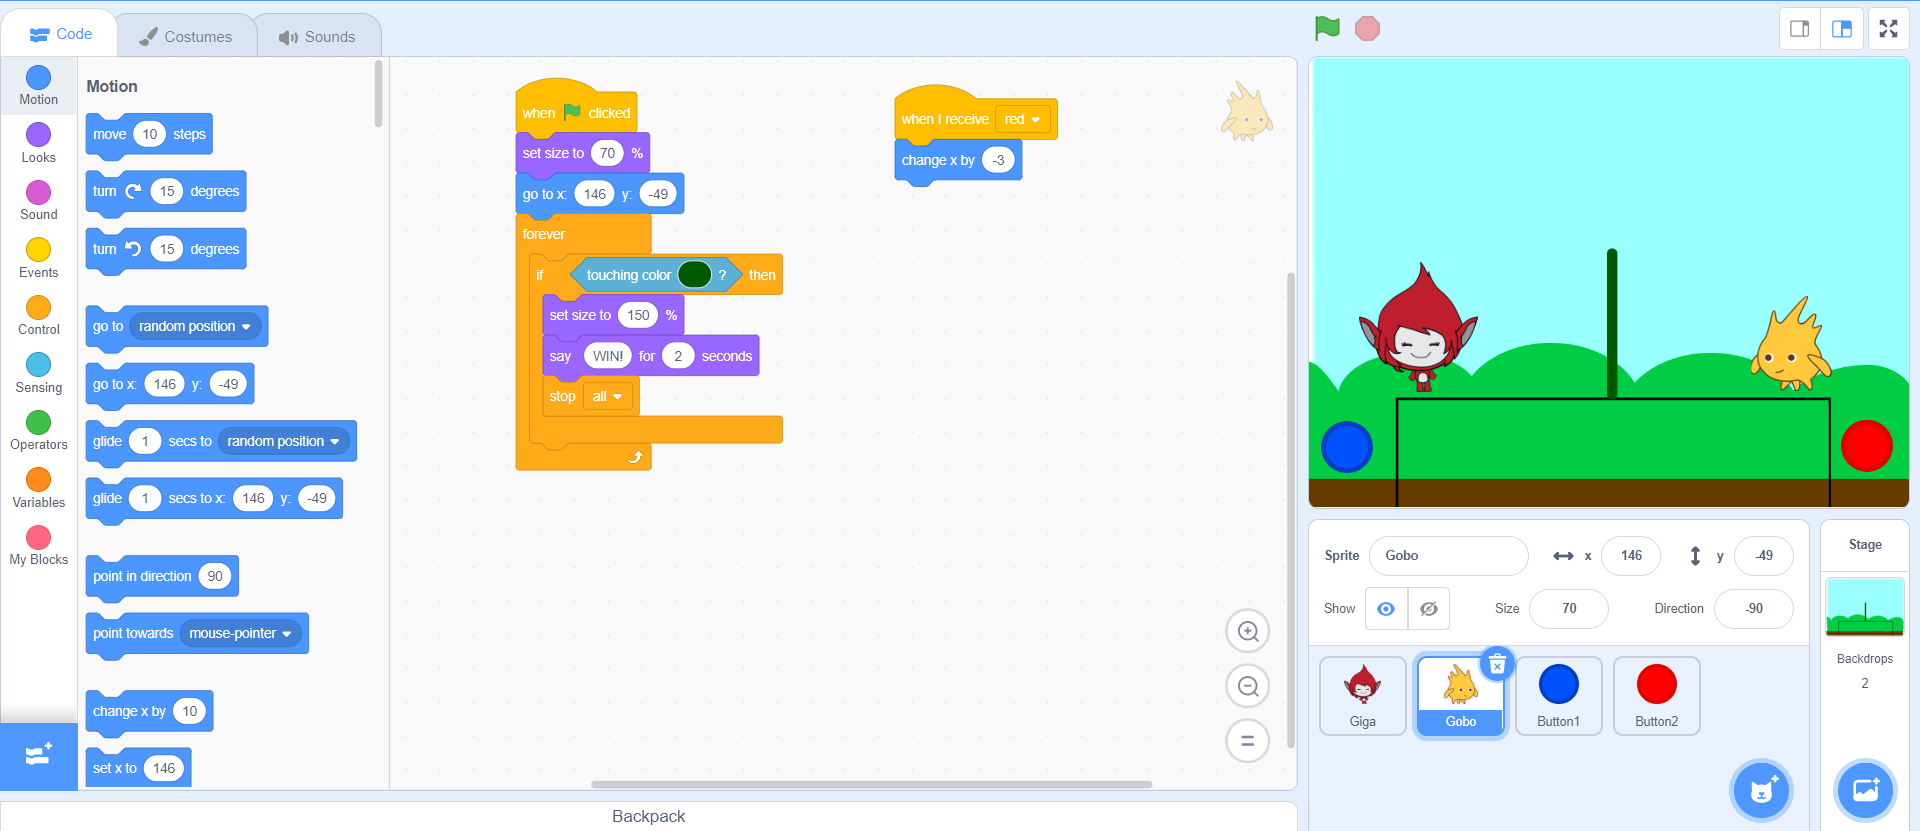
\includegraphics[width=1.0\linewidth,height=0.5\linewidth]{fig030022.png}
  \caption{Финален код на десния герой}
\label{fig030022}
\end{figure}

Време е за забавление заедно с приятели и съпоставяне на силите, за това кой герой по- бързо ще достигне до финала.